\documentclass{article}
\PassOptionsToPackage{numbers,sort&compress}{natbib}
\usepackage[main]{neurips_2026}
\usepackage[utf8]{inputenc}
\usepackage[T1]{fontenc}
\usepackage{courier} % scalable embedded monospace; avoids bitmap Type3 fonts
\usepackage{amsmath,amssymb,amsthm,booktabs,graphicx,longtable}
\usepackage{hyperref,url,microtype,xcolor}
\newtheorem{theorem}{Theorem}
\newtheorem{proposition}{Proposition}
\newtheorem{lemma}{Lemma}
\newcommand{\E}{\mathbb E}
\newcommand{\Var}{\operatorname{Var}}
\newcommand{\Cov}{\operatorname{Cov}}
\newcommand{\CP}{\operatorname{CP}}
\newcommand{\SharpSafeCov}{100.0}
\newcommand{\SharpSafeWidth}{0.0644}
\newcommand{\SharpSafeRatioPP}{0.735}
\newcommand{\SharpSafeGainPP}{26.5}
\newcommand{\SharpSafeRatioLabel}{0.720}
\newcommand{\SharpSafeGainLabel}{28.0}
\newcommand{\SharpCPCov}{100.0}
\newcommand{\SharpCPWidth}{0.0538}
\newcommand{\SharpCPRatioPP}{0.614}
\newcommand{\SharpCPGainPP}{38.6}
\newcommand{\SharpCPRatioLabel}{0.602}
\newcommand{\SharpCPGainLabel}{39.8}
\newcommand{\SharpLargeCov}{100.0}
\newcommand{\SharpLargeWidth}{0.0292}
\newcommand{\SharpLargeRatioPP}{0.666}
\newcommand{\SharpLargeGainPP}{33.4}
\newcommand{\SharpLargeRatioLabel}{0.659}
\newcommand{\SharpLargeGainLabel}{34.1}
\newcommand{\RarePPCov}{62.6}
\newcommand{\RarePPWidth}{0.0245}
\newcommand{\RarePPRatioPP}{1.000}
\newcommand{\RarePPGainPP}{0.0}
\newcommand{\RarePPRatioLabel}{0.470}
\newcommand{\RarePPGainLabel}{53.0}
\newcommand{\RareLabelCov}{98.2}
\newcommand{\RareLabelWidth}{0.0521}
\newcommand{\RareLabelRatioPP}{2.127}
\newcommand{\RareLabelGainPP}{-112.7}
\newcommand{\RareLabelRatioLabel}{1.000}
\newcommand{\RareLabelGainLabel}{0.0}
\newcommand{\ShiftPPCov}{0.0}
\newcommand{\ShiftPPWidth}{0.0008}
\newcommand{\ShiftPPRatioPP}{1.000}
\newcommand{\ShiftPPGainPP}{0.0}
\newcommand{\ShiftPPRatioLabel}{0.009}
\newcommand{\ShiftPPGainLabel}{99.1}
\newcommand{\ShiftHalfCov}{0.0}
\newcommand{\ShiftHalfWidth}{0.1494}
\newcommand{\ShiftHalfRatioPP}{192.666}
\newcommand{\ShiftHalfGainPP}{-19166.6}
\newcommand{\ShiftHalfRatioLabel}{1.672}
\newcommand{\ShiftHalfGainLabel}{-67.2}
\newcommand{\ShiftSafeCov}{98.9}
\newcommand{\ShiftSafeWidth}{0.1132}
\newcommand{\ShiftSafeRatioPP}{145.967}
\newcommand{\ShiftSafeGainPP}{-14496.7}
\newcommand{\ShiftSafeRatioLabel}{1.267}
\newcommand{\ShiftSafeGainLabel}{-26.7}
\newcommand{\GalaxySafeCov}{99.1}
\newcommand{\GalaxySafeWidth}{0.0994}
\newcommand{\GalaxySafeRatioPP}{1.873}
\newcommand{\GalaxySafeGainPP}{-87.3}
\newcommand{\GalaxySafeRatioLabel}{1.266}
\newcommand{\GalaxySafeGainLabel}{-26.6}
\newcommand{\ForestSafeCov}{99.3}
\newcommand{\ForestSafeWidth}{0.0817}
\newcommand{\ForestSafeRatioPP}{1.529}
\newcommand{\ForestSafeGainPP}{-52.9}
\newcommand{\ForestSafeRatioLabel}{1.265}
\newcommand{\ForestSafeGainLabel}{-26.5}
\newcommand{\SmoothFourCov}{94.8}
\newcommand{\SmoothFourWidth}{0.0371}
\newcommand{\SmoothFourRatioPP}{0.888}
\newcommand{\SmoothFourGainPP}{11.2}
\newcommand{\SmoothFourRatioLabel}{0.878}
\newcommand{\SmoothFourGainLabel}{12.2}
\newcommand{\MinExactCoverage}{94.3}
\newcommand{\MaxExactWidthSE}{0.00045}
\newcommand{\MinExactSimLower}{92.7}
\newcommand{\NumUndercoverage}{31}
\newcommand{\TotalTrialInputs}{103500}
\newcommand{\MainRuntime}{39.1}
\newcommand{\SupplementRuntime}{7.8}

\title{Interval-Width Headroom with Fixed Predictions:\\A Finite-Sample Audit of Nonlinear Score Information}
\author{Anonymous research draft}

\begin{document}
\maketitle
\begin{abstract}
Can a confidence interval be shortened without acquiring labels, adding unlabeled observations, or changing a predictor? We study binary population means with identical inputs shared across methods. A control-variance decomposition identifies nonlinear conditional-mean information that a scalar power-tuned correction cannot use; the headroom vanishes for affine conditional means within this estimator family. To separate that headroom from finite-sample validity, we construct conservative intervals by exact binomial inversion for both stratum responses and unknown stratum masses, with simultaneous protection for partition selection. We audit \TotalTrialInputs{} paired trial inputs. In a nearly deterministic nonlinear example at 500 labels, the selection-protected interval is \SharpSafeGainPP{}\% narrower than PPI++, with zero observed misses in 3,000 repetitions. This is a conditional result: it is wider on both supplied real-data prediction pools, and selection, sparse strata, and finite unlabeled budgets can erase the gain. Rare-outcome Wald intervals attain only \RarePPCov{}\% coverage at 100 labels, illustrating why shorter is not necessarily better. The contribution is a reproducible validity--width audit, not a new debiasing principle or a universal improvement theorem.
\end{abstract}

\section{Introduction}
A scientific analyst may inherit a small labeled sample, a larger unlabeled sample, and an immutable prediction rule. Prediction-powered inference (PPI) uses the labels to correct prediction bias while exploiting the prediction average \citep{ppi}. Power tuning can protect against an unhelpful scalar prediction \citep{ppiplus}. Neither development makes the question of remaining interval-width headroom vacuous: an informative score can have zero linear correlation with the response, finite unlabeled samples introduce uncertainty, and finite-sample coverage need not follow from an asymptotic theorem.

We ask a narrower, falsifiable question: \emph{for a binary population mean, when does nonlinear information in the same fixed score allow shorter intervals, after accounting for estimated score-stratum masses, selection, and coverage?} We select a mean because it directly represents a scientific prevalence, its truth can be known in simulation, and it admits both exact binomial inference and transparent variance algebra. We do not target a realized sample mean or an individual prediction interval. The real-data evaluation below conditions on two finite empirical populations; it is not deployment validation.

The analysis separates three issues often conflated in an efficiency comparison. First, a score may retain information outside its best affine projection. Second, an estimator may learn to exploit that information, yet its Wald interval can under-cover at small sample sizes. Third, a finite-sample interval can retain coverage but lose the apparent width gain to mass estimation and multiple comparisons. We evaluate these issues on exactly the same labeled and unlabeled inputs in each repetition; no label allocation, extra labels, predictor training, or predictor replacement occurs.

The resulting contributions are deliberately modest. We (i) give an explicit scalar-versus-nonlinear variance identity and its no-headroom condition within a stated control family; (ii) spell out a conservative, implementable finite-sample interval for fixed score partitions with unknown masses and protected partition selection; and (iii) provide a paired audit with negative controls, exact and asymptotic baselines, Monte Carlo uncertainty, and reproducible failures. The statistical ingredients are classical, and stratification already appears in prediction-powered inference \citep{stratppi}. We make no priority claim for score postprocessing, stratification, binomial inversion, or simultaneous selection, and no claim to exhaustive novelty clearance.

\section{Setting and existing methods}\label{sec:setting}
Let $(Y_i,S_i)_{i=1}^n$ and $(\widetilde S_j)_{j=1}^N$ be independent iid samples from the same population, where $Y\in\{0,1\}$ and $S=f(X)\in[0,1]$. The base rule $f$ is fixed independently of these evaluation samples. Our estimand is $\mu=\E Y$. ``Fixed data'' means that all competing methods receive the same realized inputs within a trial; frequentist coverage is over repetitions of the sampling process. Once all observations and all algorithmic choices are conditioned on, a deterministic interval has no nontrivial repeated-sampling coverage probability left to evaluate.

For a deterministic square-integrable control $h$, define
\begin{equation}\label{eq:control}
 \widehat\mu_h=\overline Y_L+\overline h_U-\overline h_L,\qquad
 V_h=\frac{\Var(Y-h(S))}{n}+\frac{\Var(h(S))}{N}.
\end{equation}
This estimator is unbiased for every fixed $h$, not only accurate predictions. Classical inference uses $h=0$; the original mean PPI estimator uses $h(S)=S$ \citep[Algorithm 1]{ppi}. The common mean PPI interval is a Wald interval with the two variances in \eqref{eq:control} estimated empirically. Its general validity is asymptotic. PPI also gives a finite-sample framework from valid component sets \citep[Theorem 1]{ppi}; finite-sample PPI is not a new idea introduced here.

For scalar power tuning, $h(S)=\lambda S$, PPI++ uses the consistent plug-in
\begin{equation}\label{eq:lambda}
 \widehat\lambda=\frac{\widehat\Cov_L(Y,S)}{(1+n/N)\widehat\Var_{L\cup U}(S)}.
\end{equation}
The denominator pools both score samples, as in \citet[Example 6.1]{ppiplus}. We use unrestricted real $\lambda$, including negative values: the mean objective remains convex, so clipping to $[0,1]$ is unnecessary. A constant score receives $\widehat\lambda=0$. PPI++'s asymptotic efficiency improvement is not a finite-sample no-worse-width guarantee. We use unbiased empirical variance divisors throughout, rather than the original PPI algorithm's divisors $n,N$; this does not change first-order limits.

\paragraph{Stratification and scope.}
\citet[Section 4]{stratppi} study fixed within-stratum sample sizes and stratum weights, with allocation choices and asymptotic confidence intervals. Our labels arrive under iid sampling with random cell counts, and masses must be estimated from the available unlabeled sample. We neither reallocate labels to realize their design nor label our procedure a reproduction of that fixed-allocation algorithm. Fixed-score partition summaries are downstream inference, not changes to the base prediction rule. If a stronger interpretation forbids even downstream score summaries, the nonlinear route is outside that narrower problem. We consider it allowed here while keeping every base score unchanged.

\section{What nonlinear information can and cannot buy}\label{sec:oracle}
Put $r=n/N$ and $m(S)=\E[Y\mid S]$. Write $h_0=h-\E h$. The following elementary calculation locates the potential gain before any fitting or confidence-interval calibration.
\begin{proposition}[Control-family headroom]\label{prop:oracle}
Under the assumptions of Section~\ref{sec:setting},
\begin{align}
 nV_h&=\Var(Y)-\frac{\Var(m(S))}{1+r}
 +(1+r)\E\left[\left(h_0-\frac{m(S)-\mu}{1+r}\right)^2\right],\label{eq:square}\\
 V_*&=\frac{\E\Var(Y\mid S)}{n}+\frac{\Var(m(S))}{n+N}.\label{eq:oracle}
\end{align}
The minimum over fixed score-only controls is attained at $h=m/(1+r)+c$. If $\Var(S)>0$, the best scalar control has $\lambda_* =\Cov(Y,S)/[(1+r)\Var(S)]$ and
\begin{equation}\label{eq:headroom}
 V_{\rm lin}-V_*=\frac{\Var(m(S))-\Cov(Y,S)^2/\Var(S)}{n(1+r)}\geq0.
\end{equation}
Equality holds exactly when $m(S)$ is affine in $S$ almost surely.
\end{proposition}
\paragraph{Proof idea.}
$Y-m(S)$ is orthogonal to every square-integrable score function. Expanding $\Var(Y-h)+r\Var(h)$ and completing a square gives \eqref{eq:square}; minimizing the scalar quadratic gives \eqref{eq:headroom}. Cauchy--Schwarz yields nonnegativity and the affine equality condition. Complete proofs are in Appendix~\ref{app:proofs}.

The result is \emph{not} a global impossibility theorem for confidence-interval shortening. Affine $m$ leaves no first-order oracle headroom over the optimal scalar within \eqref{eq:control}, but higher-order calibration or a different estimator class is not ruled out. If $m$ is constant, the optimum is labeled-only variance; if $S$ is constant, every score contrast vanishes. A large gap in \eqref{eq:headroom} is an opportunity, not evidence that a feasible estimated interval will improve.

For a fixed partition $B=B(S)$, let $m_B=\E[Y\mid B]$. Restricting controls to its bin indicators replaces $m$ by $m_B$, with approximation loss $\E[(m-m_B)^2]/[n(1+r)]$. Refining a partition weakly reduces this oracle loss, but arbitrary increases in bin count do not. A bin-control class also need not contain the scalar score. None of these approximation statements orders finite-sample interval widths.

Our asymptotic nonlinear baseline estimates each bin response mean using \emph{all} labels and sets $\widehat h_k=\widehat p_k/(1+n/N)$. With a fixed finite number of independent, prespecified boundaries, positive active cell masses, and $n/N\to\rho<\infty$, its fitted-control remainder is $o_p(n^{-1/2})$. For the residual/unlabeled plug-in variance, $n\widehat V\to_p v_\rho$; a Wald theorem requires $v_\rho>0$. Thus cross-fitting is not required for this fixed-dimensional construction, but sparse strata and zero empirical variance remain small-sample hazards. The proof and degenerate cases appear in Appendix~\ref{app:plugin}; no finite-sample unbiasedness is claimed for the fitted map.

\section{Finite-sample intervals with unknown stratum masses}\label{sec:exact}
A simple exact-in-coverage construction makes the validity cost explicit. Fix a partition $A_1,\ldots,A_K$ independently of both evaluation samples. Let $C_k,T_k$ be its labeled cell count and success count; let $D_k$ be its unlabeled count. Write $p_k=P(Y=1\mid S\in A_k)$, $w_k=P(S\in A_k)$, so $\mu=\sum_k w_kp_k$. For positive weights, $T_k\mid(C_1,\ldots,C_K)\sim\operatorname{Bin}(C_k,p_k)$ and $D_k\sim\operatorname{Bin}(N,w_k)$ marginally. This conditions on counts, \emph{not} on every realized score.

For $K\geq2$, construct equal-tailed Clopper--Pearson (CP) intervals
\begin{equation}\label{eq:cpboxes}
 [a_k,b_k]=\CP(T_k,C_k;\alpha/(2K)),\qquad
 [\ell_k,u_k]=\CP(D_k,N;\alpha/(2K)).
\end{equation}
Here the third argument is total two-sided error. Empty labeled cells receive $[0,1]$; cells of population mass zero can have arbitrary $p_k$. Define
\begin{equation}\label{eq:lp}
 \mathcal W=\{v:\ell_k\leq v_k\leq u_k,\ \sum_kv_k=1\},\quad
 I_B=\left[\min_{v\in\mathcal W}\sum_ka_kv_k,\ \max_{v\in\mathcal W}\sum_kb_kv_k\right].
\end{equation}
For $K=1$, use labeled-only CP at error $\alpha$, without wasting an error budget on a known unit mass.

\begin{theorem}[Coverage and protected selection]\label{thm:exact}
For every positive $n,N$ and every population satisfying Section~\ref{sec:setting}, $P(\mu\in I_B)\geq1-\alpha$. For a prespecified family of $M$ partitions, construct each $I_B$ at error $\alpha/M$. Selecting the shortest of these corrected intervals, with fixed tie breaking, also has coverage at least $1-\alpha$.
\end{theorem}
\paragraph{Proof idea.}
Conditional binomial inversion controls each response error even for random counts; binomial inversion also controls each mass error. A union bound covers all $2K$ components. On that event, the true $w$ is feasible in \eqref{eq:lp}, and $a\leq p\leq b$, so the endpoints enclose $\mu$. CP contains each observed proportion, so $D/N\in\mathcal W$ and the optimization is always feasible. Another union bound protects arbitrary selection over the prespecified family. No independence among component intervals or among candidates is needed. Appendix~\ref{app:proofs} supplies the details.

Both endpoint optimizations are solved by filling the box-constrained simplex in order of the objective coefficients. Our implementation additionally evaluates the corresponding dual bound with outward padding, avoiding reliance on approximate primal feasibility. Standard double-precision beta quantiles are padded outwards; we do not claim formal certification of library special-function error. The theorem is a real-arithmetic statistical guarantee, not a machine-verified floating-point theorem.

The selector, called \textbf{Safe CP}, uses four fixed partitions: one bin, score halves, a tails-versus-center split at $1/4,3/4$, and four equal score bins. Each candidate receives $\alpha/4$. The standalone \textbf{Tails CP} uses the tails partition at error $\alpha$. Protected selection is no wider than its corrected candidates, but need not beat an uncorrected labeled CP or PPI++ interval. Choosing the shortest ordinary 95\% candidate (``unsafe selection'') has no analogous coverage argument, even if a simulation happens to look conservative.

\section{Experiments}\label{sec:experiments}
\subsection{Paired protocol and uncertainty}
All intervals have nominal level 95\%. Main synthetic experiments use $n\in\{100,500,2000\}$, $N=20n$, and 3,000 independent repetitions per cell, divided into seeds 1729, 2027, 7919. Sensitivity experiments use $n=500$, $N/n\in\{1,5,100\}$, and 1,500 repetitions for affine, sharp-tail, and irrelevant scores. Two fixed real-data prediction pools use the main budgets. There are 39 cells and \TotalTrialInputs{} distinct paired trial inputs, not that many independent datasets or trained predictors. Fourteen original methods plus two descriptive Hoeffding supplements give 1,656,000 method-output rows. All methods receive identical labeled outcomes and scores and identical unlabeled scores within each repetition. Algorithms never receive unlabeled outcomes.

The fixed synthetic laws use labeled $S\sim U[0,1]$ and Bernoulli $Y$ with the conditional means in Appendix~\ref{app:protocol}. Affine and reversed-affine laws have $m(s)=.05+.9s$ and $.95-.9s$. Smooth U uses $.05+.9(2s-1)^2$. Sharp tails uses $.005+.99\mathbf1\{s<.25\text{ or }s\geq.75\}$; its known mean is $.5$. Irrelevant and constant scores have outcome mean $.35$. Rare tails has mean $.01$. A shift stress test changes only unlabeled scores to $\operatorname{Beta}(4,1)$, violating the common-population assumption. No scenario was dropped after observing outcomes.

\paragraph{Baselines.}
We compare labeled Wald and CP, original PPI Wald, unrestricted PPI++, full-data fixed-bin Wald controls (half, tails, four and eight bins), standalone fixed-partition CP, Safe CP, unsafe selection, and infeasible known-mass CP. An audit, after mechanics-only smoke checks and declared before full outcome inspection, added labeled Hoeffding and original PPI's union-Hoeffding specialization as descriptive finite-sample baselines; they are not in the locked testing families. An exploratory post-audit mass ablation is separately labeled below. All reported intervals are clipped to $[0,1]$; zero empirical variance gives a point Wald interval rather than silently removing a repetition.

Coverage error bars are pointwise Wilson 95\% Monte Carlo (MC) intervals. Mean-width error bars use $1.96$ MC standard errors. Width ratios are ratios of mean widths with a paired delta-method MC interval, not means of per-trial ratios. A declared family of 72 one-sided paired width tests (Safe CP versus PPI++, Tails CP versus labeled CP in 36 nonshift cells) uses Holm correction. Exact binomial undercoverage tests use a separate 252-test Holm family for seven asymptotic methods; exact simultaneous MC lower bounds use a separate 180-member family. These families and their timing are documented in the supplement. Pointwise ratio intervals do not become simultaneous merely because a related width test is adjusted.

\subsection{Synthetic headroom and its costs}
\begin{table}[t]
\centering\small
\caption{Main synthetic results at $n=500,N=10{,}000$. Each entry is mean width / coverage in percent (3,000 repetitions). These are not equal-validity width rankings: CP procedures have finite-sample guarantees under assumptions; Wald procedures are asymptotic. Complete MC uncertainty is in Appendix~\ref{app:allresults}.}\label{tab:main}
\begin{tabular}{lrrrrr}
\toprule
Scenario & Label CP & PPI++ & Bin4 Wald & Tails CP & Safe CP \\
\midrule
Affine & 0.0893 / 95.6 & 0.0755 / 95.2 & 0.0761 / 95.1 & 0.1615 / 99.9 & 0.1132 / 99.0 \\
Reversed & 0.0893 / 96.1 & 0.0755 / 94.4 & 0.0761 / 94.0 & 0.1614 / 100.0 & 0.1132 / 99.1 \\
Smooth U & 0.0853 / 95.8 & 0.0835 / 95.0 & 0.0740 / 94.8 & 0.1444 / 100.0 & 0.1081 / 99.1 \\
Sharp tails & 0.0893 / 95.8 & 0.0876 / 95.2 & 0.0226 / 94.9 & 0.0538 / 100.0 & 0.0644 / 100.0 \\
Irrelevant & 0.0853 / 95.9 & 0.0835 / 95.3 & 0.0833 / 95.1 & 0.1542 / 100.0 & 0.1080 / 99.0 \\
Constant & 0.0853 / 95.8 & 0.0836 / 95.2 & 0.0836 / 95.2 & 0.1085 / 99.2 & 0.1080 / 99.0 \\
Rare tails & 0.0195 / 97.5 & 0.0166 / 86.6 & 0.0165 / 86.6 & 0.0354 / 99.8 & 0.0246 / 99.5 \\
\bottomrule
\end{tabular}
\end{table}

Table~\ref{tab:main}, Figure~\ref{fig:main}, and paired intervals in Table~\ref{tab:paired} show the intended conditional result. For sharp tails, $\Cov(Y,S)=0$ but the tails indicator is almost a sufficient response predictor. At 500 labels, Safe CP is \SharpSafeGainPP{}\% narrower than PPI++; the pointwise paired MC interval for the reduction is $[26.28,26.75]\%$. Its observed coverage is 3,000/3,000, not a claim that its true coverage equals one. Standalone Tails CP is \SharpCPGainLabel{}\% narrower than labeled CP. At 2,000 labels the Safe CP reduction versus PPI++ is \SharpLargeGainPP{}\%. All nine Holm-significant designated width improvements occur in sharp-tail cells; no broad superiority follows.

In smooth U, Bin4 Wald realizes a \SmoothFourGainPP{}\% reduction at 2,000 labels, with \SmoothFourCov{}\% observed coverage, whereas conservative CP gains disappear. On affine and reversed-affine laws, the scalar oracle already captures the relevant conditional mean. Binned Wald controls do not improve first-order efficiency there, and simultaneous exact inference is substantially wider. Irrelevant and constant scores likewise provide no useful headroom. These are retained negative results, not failed cases removed from the comparison.

\begin{figure}[t]
\centering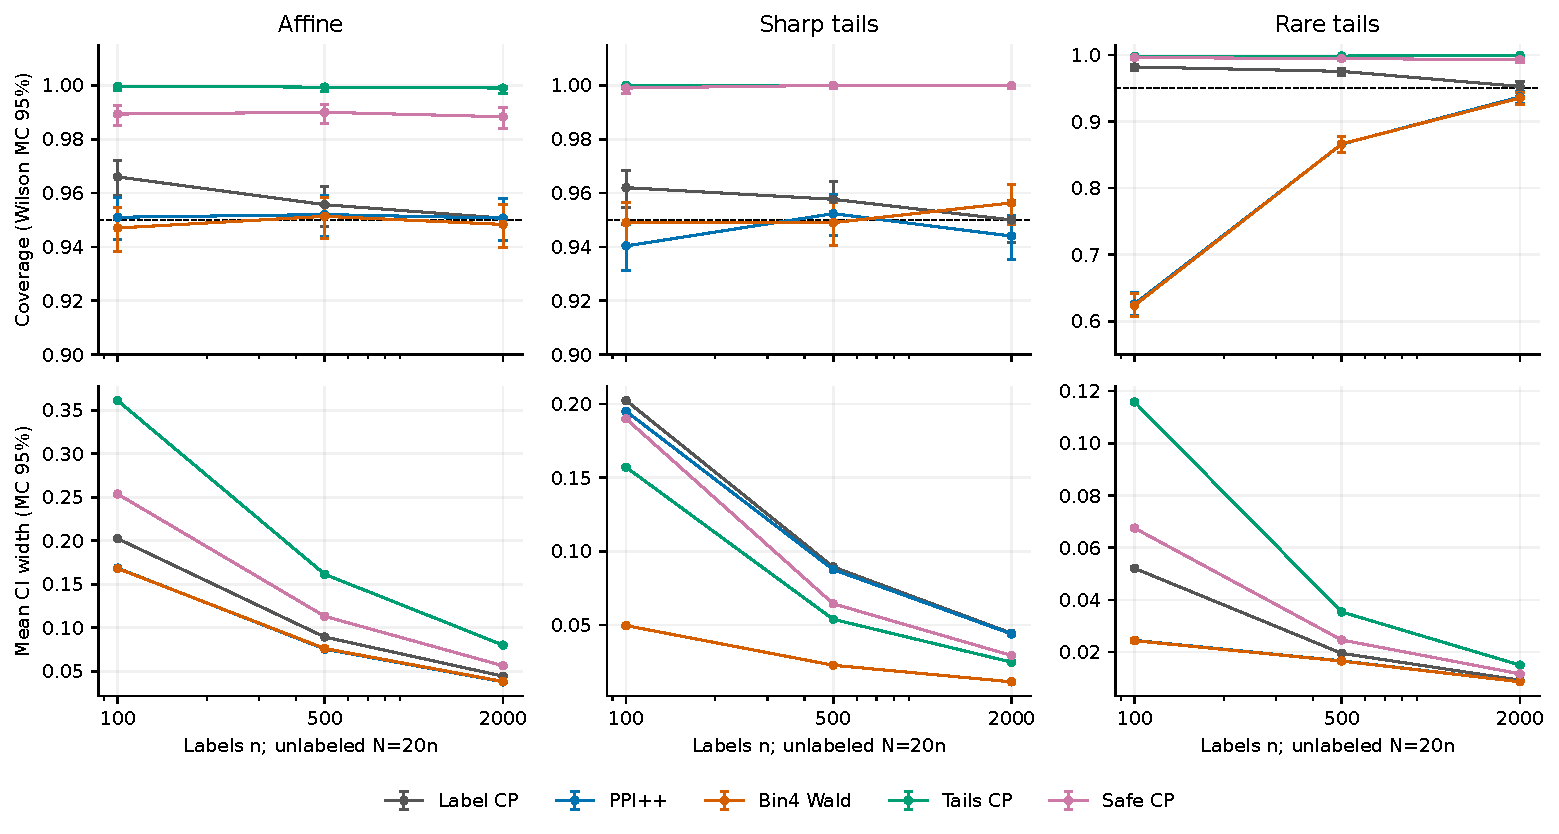
\includegraphics[width=\linewidth]{figures/coverage_width.pdf}
\caption{Coverage (top) and width (bottom) on three prespecified laws. Coverage bars are pointwise Wilson MC95; width bars are $1.96$ MCSE. Exact construction costs precision on affine data, exploits sharp nonlinear information, and avoids the rare-event Wald collapse. Near-invisible width bars reflect precise MC means, not certainty about future scientific populations.}\label{fig:main}
\end{figure}

\paragraph{Finite unlabeled data and selection are not free.}
At sharp tails and $n=500$, Safe CP/PPI++ mean-width ratios are $1.292,1.061,.735,.554$ for $N/n=1,5,20,100$. The gain reverses at limited unlabeled budgets in this grid; these four points do not estimate a universal crossover. Figure~\ref{fig:sensitivity} shows this dependence. All same-population exact-family observed coverages range down to \MinExactCoverage{}\%, from labeled CP; the minimum simultaneous MC lower bound is \MinExactSimLower{}\%, not 95\%. Finite MC frequencies need not exceed nominal coverage in every cell. The three observed exact-method rates below 95\% are statistically compatible with nominal after considering their uncertainty; the mathematical proof, not this observation, supplies the finite-sample guarantee.

\begin{table}[t]
\centering\small
\caption{Selected paired ratios with pointwise MC95 intervals. Denominator is labeled CP for the first and fifth rows, PPI++ otherwise. Coverage columns also have pointwise Wilson MC95. Asymptotic Bin4 and finite-sample CP rows have different guarantees; the smooth-U row is descriptive, not a designated width test.}\label{tab:paired}
\begin{tabular}{llrrrr}
\toprule Case & Method & Width ratio & Ratio MC 95\% & Coverage & MC 95\% \\\midrule
Sharp tails 500 & Tails CP & 0.602 & [0.60005,0.60418] & 1.000 & [0.999,1.000] \\
Sharp tails 500 & Safe CP & 0.735 & [0.73255,0.73720] & 1.000 & [0.999,1.000] \\
Sharp tails 2000 & Safe CP & 0.666 & [0.66421,0.66738] & 1.000 & [0.999,1.000] \\
Smooth U 2000 & Bin4 Wald & 0.888 & [0.88736,0.88803] & 0.948 & [0.939,0.955] \\
Irrelevant 500 & Safe CP & 1.266 & [1.26647,1.26647] & 0.990 & [0.986,0.993] \\
Galaxies 500 & Safe CP & 1.873 & [1.86994,1.87558] & 0.991 & [0.987,0.994] \\
\bottomrule\end{tabular}
\end{table}

\subsection{Real prediction pools: no exact width win demonstrated}
We use the supplied \texttt{ppi-python} v0.2.3 forest and galaxies arrays, with 1,596 and 16,743 records. Labels are binary and scores are existing predictions; neither predictor is retrained. Each fixed pool defines an empirical population whose target is its exact label proportion. Labeled and unlabeled observations are drawn independently \emph{with replacement} from this population; source-record overlap does not break independence of independent draws. This identifies repeated-sampling coverage for that empirical law, not the original forest or galaxy superpopulation, and does not create new unique source information. The predictors' original training independence cannot be re-audited from these arrays.

Table~\ref{tab:real} and Figure~\ref{fig:real} report the negative result. At 500 labels, Safe CP is 52.9\% wider than PPI++ for forest and 87.3\% wider for galaxies. In both cells it always selects the multiplicity-adjusted labeled candidate. It is also wider than ordinary labeled CP. Nonlinear finite-sample gains in the sharp-tail construction therefore do not transfer to these pools. PPI++ has significant adjusted undercoverage at 100 labels in both datasets, however, so its shorter width is not a universal finite-sample validity result either.

\begin{table}[t]
\centering\small
\caption{Fixed real-prediction empirical populations: mean width / coverage percent. All cells have 3,000 repetitions, $N=20n$. Repeated source records at large $n,N$ reflect empirical-population sampling, not additional collected data.}\label{tab:real}
\begin{tabular}{llrrrrr}
\toprule
Data & $n$ & Label CP & PPI++ & Bin4 Wald & Tails CP & Safe CP \\
\midrule
Forest & 100 & 0.1485 / 94.4 & 0.1200 / 92.3 & 0.1179 / 92.0 & 0.2488 / 100.0 & 0.1858 / 99.0 \\
Forest & 500 & 0.0646 / 96.1 & 0.0535 / 94.5 & 0.0540 / 94.4 & 0.1117 / 100.0 & 0.0817 / 99.3 \\
Forest & 2000 & 0.0319 / 95.4 & 0.0268 / 95.0 & 0.0272 / 95.5 & 0.0554 / 99.9 & 0.0405 / 98.4 \\
Galaxies & 100 & 0.1785 / 95.3 & 0.1187 / 93.4 & 0.1172 / 92.8 & 0.3034 / 100.0 & 0.2236 / 99.2 \\
Galaxies & 500 & 0.0785 / 94.9 & 0.0531 / 94.4 & 0.0539 / 94.4 & 0.1372 / 100.0 & 0.0994 / 99.1 \\
Galaxies & 2000 & 0.0389 / 95.7 & 0.0265 / 94.3 & 0.0271 / 94.8 & 0.0682 / 100.0 & 0.0494 / 99.3 \\
\bottomrule
\end{tabular}
\end{table}

\subsection{Failures and ablations}
\paragraph{Zero labels and shift expose different collapses.}
Rare tails at $n=100$ gives PPI++ coverage \RarePPCov{}\%, versus \RareLabelCov{}\% for labeled CP. Its 1,121 intervals $[0,0]$ account for all but one miss: with zero observed successes the fitted covariance and variance both vanish. The population all-zero probability is $.99^{100}$, so this is a predictable failure mechanism rather than evidence of extra information. There are \NumUndercoverage{} Holm-significant undercoverage tests across the 252 asymptotic cells/methods, with eight-bin controls particularly fragile at small $n$. Figure~\ref{fig:bins} displays the corresponding bin-complexity width comparison; its coverage must still be checked separately.

Under the deliberate score-distribution shift at $n=500$, PPI++ covers in zero trials; 2,883/3,000 intervals clip to $[1,1]$. The biased untruncated center moves beyond the support, so its tiny reported width is a clipping pathology, not efficiency. Safe CP happens to select labeled-only in this stress test; that does not extend Theorem~\ref{thm:exact} to shifted masses. Zero-label and support-clipping point intervals must not be interpreted as the same mechanism.

\paragraph{Isolating mass uncertainty.}
The original known-mass diagnostic removes mass error and reallocates its error budget to the response intervals, so its gap does \emph{not} isolate the cost of unknown masses. A post-audit exploratory rerun on identical sharp-tail inputs fixes response error at $\alpha/(2K)$ in both variants. At $n=500,N=10{,}000$, widths are $.053795$ (unknown), $.029482$ (known, matched response budget), and $.026207$ (known, reallocated). Thus the isolated mass gap is $.024313$ (paired MCSE $.000003$), with a separate reallocation gap $.003275$. This diagnostic uses true weights only as an infeasible ablation; it is not extra information available to any feasible competitor. Complete budget sensitivity is in Appendix~\ref{app:mass}, Table~\ref{tab:mass}.

\section{Discussion, limitations, and conclusion}\label{sec:discussion}
The fixed-input question has a conditional answer. A score may encode strong nonlinear information even when its scalar linear correction is useless; exploiting it can shorten a finite-sample valid interval without new data or a new predictor. Conversely, affine conditional means leave no nonlinear oracle headroom over optimal scalar control in this family. Finite-sample response uncertainty, unknown masses, protected selection, and sparse bins determine whether potential headroom survives in an actual interval.

These conclusions are restricted to binary means, independent common-population sampling, fixed independent partitions, and a small prespecified method family. Our exact construction is conservative, not a shortest-valid-interval algorithm. We have not compared every exact PPI component construction or optimized exact joint multinomial regions. No universal finite-sample dominance or impossibility theorem is established. The unrestricted conditional-mean oracle is not a feasible fitted predictor and is not claimed as a new efficiency bound. The real-data evidence concerns two empirical pools, with no deployment or predictor-training uncertainty assessment. The sharp-tail example is intentionally favorable and nearly deterministic; it is a mechanism test, not evidence of typical scientific effect sizes.

Numerical bounds use standard padded double-precision beta quantiles, not formally verified interval arithmetic. Numerical fallback counts and preclipping centers were not logged in the original runs; endpoint checks cannot prove the absence of all fallback events. Separate method timings are unavailable. The initial implementation and smoke checks, all failed analysis attempts, and the later exploratory ablation are documented rather than presented as a single preregistered study.

\paragraph{Broader impact and research process.}
Narrow but invalid intervals can create false certainty in scientific and policy decisions; conservative valid intervals can instead make fixed annotation budgets more trustworthy, at a measurable precision cost. The comparisons recommend reporting both coverage and width and disclosing distribution mismatch, rather than selecting whichever interval looks shortest. No human participants, personal records, or high-risk models were collected or released. Original data licenses were not independently resolved; the reproducibility release supplies retrieval instructions and hashes instead of redistributing the raw third-party arrays. This work was conducted by an autonomous language-model research assistant, including design, coding, analysis and drafting, with independent subagent audits; the scripts themselves make no LLM or paid API calls. This disclosure is not a claim of human-author verification.

The practical recommendation is therefore not ``always recalibrate.'' Inspect what information remains in the fixed score, pay explicitly for finite-data and selection uncertainty, and retain the labeled-only alternative. In this audit, genuine exact gains and substantial negative results coexist.

\clearpage
\bibliographystyle{plainnat}
\bibliography{references}

\clearpage
\appendix
\section{Complete proofs}\label{app:proofs}
\subsection{Binomial inversion and conditional cell counts}
For $T\sim\operatorname{Bin}(m,p)$, define the equal-tailed CP interval at error $\delta$ by
\begin{equation}\label{eq:cpformula}
 a=\begin{cases}0&T=0,\\ F^{-1}_{\operatorname{Beta}(T,m-T+1)}(\delta/2)&T>0,\end{cases}\quad
 b=\begin{cases}1&T=m,\\ F^{-1}_{\operatorname{Beta}(T+1,m-T)}(1-\delta/2)&T<m.\end{cases}
\end{equation}
For $m=0$ set $[a,b]=[0,1]$. The lower endpoint inverts the upper binomial tail and the upper endpoint inverts the lower tail. A discrete one-sided tail test at error $\delta/2$ rejects with probability at most $\delta/2$; taking the union of the two rejected tails gives $P_p(p\notin[a,b])\leq\delta$. This standard test-inversion argument also establishes conservatism at boundary probabilities.

For a fixed partition, the joint category probabilities of $(B,Y)$ are $w_kp_k,w_k(1-p_k)$. Dividing the multinomial joint mass of response and cell counts by the multinomial mass of $C=(C_1,\ldots,C_K)$ yields
\begin{equation}\label{eq:conditional}
 P(T=t\mid C=c)=\prod_k {c_k\choose t_k}p_k^{t_k}(1-p_k)^{c_k-t_k}.
\end{equation}
Thus binomial CP covers $p_k$ conditional on each possible count vector, and its unconditional error is also at most its assigned budget by total probability. Empty labeled cells are covered by convention; zero-population-mass cells are empty almost surely. The unlabeled count $D_k$ has marginal binomial law regardless of dependence among different $D_k$.

Apply these facts with $\delta=\alpha/(2K)$ to the response and mass intervals. Their union failure probability is at most $2K\delta=\alpha$. On the simultaneous coverage event, $w\in\mathcal W$ and $a_k\leq p_k\leq b_k$; because all weights are nonnegative,
\begin{equation}\label{eq:coveragechain}
 \min_{v\in\mathcal W}a^\top v\leq a^\top w\leq \mu\leq b^\top w\leq\max_{v\in\mathcal W}b^\top v.
\end{equation}
The ordinary CP interval contains the empirical proportion for every count (equivalently, the integer binomial mean is a median). Hence $D/N\in\mathcal W$, making it nonempty for every observed dataset; it is compact. This proves the fixed-partition claim including empty cells. For $K=1$ use the binomial argument directly.

For $M$ fixed candidates, each constructed at error $\alpha/M$, the probability that all cover is at least $1-\alpha$ by another union bound. On this event any selected candidate covers, even when the selector uses all data. This proves Theorem~\ref{thm:exact}. It does not protect a partition collection first chosen using evaluation data without including those choices in the simultaneous family.

\subsection{Box-simplex optimization and dual bounds}
For a cost vector $c$, start with $v=\ell$ and residual $R=1-\sum_k\ell_k$. Allocate mass, up to each capacity $u_k-\ell_k$, in ascending order of $c_k$. Feasibility follows from $\sum\ell\leq1\leq\sum u$. If a feasible vector puts transferable mass on a more expensive coordinate while a cheaper coordinate has unused capacity, transferring $\varepsilon$ decreases the objective by $\varepsilon(c_j-c_i)$. Repeated exchanges give the sorted-fill solution, proving the minimum; descending order proves the maximum.

A useful numerical certificate does not require exact primal feasibility. For every real $\lambda$ and feasible $v$,
\begin{equation}\label{eq:dualmin}
 c^\top v\geq\lambda+\sum_k(c_k-\lambda)\begin{cases}\ell_k&c_k\geq\lambda,\\u_k&c_k<\lambda,\end{cases}
\end{equation}
since $\sum v_k=1$ and each summand is separately minimized over its box. Replacing minima by maxima gives a universal upper bound. The greedy threshold supplies an optimal $\lambda$ in exact arithmetic; an approximate threshold still supplies a valid dual bound in exact arithmetic. Code pads component and final endpoints outward by $10^{-10}$ and fails to $[0,1]$ if its feasibility/finite checks fail. The number of bins is at most eight, so ordinary objective rounding is far below this pad for inputs in $[0,1]$. Special-function quantile error has not been formally enclosed, and the statistical theorem is not represented as a formal software proof.

\subsection{Proof of Proposition~\ref{prop:oracle}}
Conditional expectation gives $\Cov(Y,h(S))=\E[(m(S)-\mu)h_0]$. Independence of the two samples proves \eqref{eq:control}; expanding its variance gives
\begin{equation}\label{eq:expand}
 nV_h=\Var(Y)-2\E[(m-\mu)h_0]+(1+r)\E h_0^2.
\end{equation}
Completing the square proves \eqref{eq:square}, with equality at $h_0=(m-\mu)/(1+r)$. Substituting the law of total variance proves \eqref{eq:oracle}. Restricting to $h=\lambda S$ minimizes a scalar quadratic and gives the stated $\lambda_*$, with minimum $nV_{\rm lin}=\Var(Y)-\Cov(Y,S)^2/[(1+r)\Var(S)]$. Subtracting \eqref{eq:oracle} gives \eqref{eq:headroom}. Since $\Cov(Y,S)=\Cov(m(S),S)$, Cauchy--Schwarz proves nonnegativity; its equality condition for $\Var(S)>0$ is $m-\mu=c(S-\E S)$ almost surely, including $c=0$. If $S$ is constant, every score function is constant, and the correction vanishes.

For bin-measurable controls, repeat the argument with $m_B=\E[Y\mid B]$. Orthogonality of conditional expectation gives $\Var(m)-\Var(m_B)=\E[(m-m_B)^2]$, proving the approximation loss. If $B'$ refines $B$, then $\E[m_{B'}\mid B]=m_B$ and $\Var(m_{B'})=\Var(m_B)+\E[(m_{B'}-m_B)^2]$. This is the precise refinement ordering, not an ordering by bin count alone. For example, $Y=\mathbf1\{S<1/2\}$ under uniform scores has zero approximation loss with halves but squared approximation error $1/12$ (variance loss $1/[12n(1+r)]$) with equal thirds. Furthermore the binned indicator span need not contain $S$, so $V^*_B$ need not dominate $V_{\rm lin}$.

\section{Fitted means on fixed bins: assumptions and degeneracies}\label{app:plugin}
This result does not learn boundaries. Fix $K<\infty$, discard zero-population-mass cells (which never appear), and assume $w_k>0$ on each active cell. Let $n,N\to\infty$ with $r_n=n/N\to\rho\in[0,\infty)$. Set $\widehat p_k=T_k/C_k$ when $C_k>0$, with global labeled mean fallback otherwise, and $\widehat h_k=\widehat p_k/(1+r_n)$. The corresponding deterministic oracle control is $h_{n,k}=p_k/(1+r_n)$.

The probability of an empty active cell is at most $\sum_k(1-w_k)^n\to0$. For nonempty cells,
\begin{equation}\label{eq:nuisance}
 \widehat p_k-p_k=\frac{n^{-1}\sum_i\mathbf1\{B_i=k\}(Y_i-p_k)}{C_k/n}=O_p(n^{-1/2}).
\end{equation}
The bounded fallback on an exponentially rare event does not change this rate. Because $K$ is fixed and $r_n$ bounded,
\begin{equation}\label{eq:remainder}
 \widehat\mu_{\widehat h}-\widehat\mu_{h_n}
 =\frac{1}{1+r_n}\sum_k(\widehat p_k-p_k)(D_k/N-C_k/n)
 =O_p(n^{-1})=o_p(n^{-1/2}).
\end{equation}
No independence between the factors in this product is required. Same-sample fitting therefore causes no first-order change; the fitted estimator need not be exactly unbiased.

Write $\sigma_e^2=\E\Var(Y\mid B)$, $\sigma_m^2=\Var(p_B)$, and $v_\rho=\sigma_e^2+\rho\sigma_m^2/(1+\rho)$. Replacing $h_n$ by $h_\rho=p/(1+\rho)$ changes the estimator by $o_p(n^{-1/2})$, because the coefficient change is $o(1)$ times a bin-frequency contrast. Two independent bounded-sample CLTs then yield
\begin{equation}\label{eq:binclt}
 \sqrt n(\widehat\mu_{\widehat h}-\mu)\ \Rightarrow\ \mathcal N(0,v_\rho).
\end{equation}
Define the centered, unbiased sample variance estimator
\begin{equation}\label{eq:variance}
 \widehat V=\frac{s_L^2(Y-\widehat h(B))}{n}+\frac{s_U^2(\widehat h(B))}{N}.
\end{equation}
Uniform consistency across the finite collection of bin values, boundedness, and the LLN for fixed-$h_\rho$ moments imply
\begin{equation}\label{eq:scaledconsistency}
 n\widehat V=s_L^2(Y-\widehat h)+r_ns_U^2(\widehat h)\ \to_p\
 \Var(Y-h_\rho)+\rho\Var(h_\rho)=v_\rho.
\end{equation}
Unscaled convergence of $\widehat V$ to zero alone would not suffice. If $v_\rho>0$, Slutsky gives asymptotically nominal studentized Wald coverage. There is no uniform assertion over growing $K$, shrinking cell masses, or population sequences.

If $v_\rho=0$ with $\rho>0$, both variance components vanish; $Y$ is constant, so a point interval covers with probability one rather than possessing a nondegenerate normal limit. If $\rho=0$ and $\sigma_e^2=0$, binary $Y$ is deterministic within each active cell. Once all cells are occupied, fitted values equal the true $p_k\in\{0,1\}$ and the estimator equals
\begin{equation}\label{eq:degeneratepooled}
 \frac{\sum_iY_i+\sum_jp_{\widetilde B_j}}{n+N}.
\end{equation}
The right side, defined with true $p$ on all datasets, is unconditionally a pooled mean of iid Bernoulli($\mu$) variables. For $0<\mu<1$ it has a $\sqrt{n+N}$ CLT, transferred to the fitted estimator by equality on an event tending to one. On the same event, $(n+N)\widehat V\to_p\mu(1-\mu)$; for $\mu\in\{0,1\}$ return to the constant case. One must not condition an iid CLT on occupancy or use only the root-$n$ remainder to assert this faster-rate result. Our experiments have $N/n$ fixed within each cell, and rare-event empirical degeneracy remains a finite-$n$ warning.

For PPI++, consistency of the ideal unrestricted scalar coefficient likewise makes its estimation error times $\overline S_U-\overline S_L$ negligible at first order. Bounded moments and $\Var(S)>0$ suffice for this ideal scalar plug-in variance argument. The code additionally zeros coefficients when the pooled score variance is at most $10^{-14}$: transferring ideal coefficient consistency to this implementation requires $\Var(S)>10^{-14}$ under common-population sampling. Below this fixed cutoff the implementation intentionally uses labeled Wald instead; at the threshold no ideal-efficiency guarantee is asserted. None of these statements makes either estimated-control Wald interval finite-sample exact.

\section{Full experimental specification}\label{app:protocol}
\subsection{Population laws and partition conventions}
Table~\ref{tab:dgps} defines every synthetic generator. Within each nonshift trial, both score samples are independently uniform except in the constant-score law; only labeled outcomes are sampled. All base scores remain immutable. Bernoulli randomization is conditionally independent across labels. The rare-tail law has mean $.001+.018/2=.01$; smooth U has mean $.05+.9/3=.35$.
\begin{table}[h]
\centering
\caption{Prespecified synthetic populations. Shift is an assumption-violation stress test, not a valid-regime efficiency benchmark.}\label{tab:dgps}
\begin{tabular}{lll}\toprule
Scenario & Labeled conditional mean $m(s)$ & Truth $\mu$\\\midrule
Affine & $.05+.9s$ & $.5$\\
Reverse & $.95-.9s$ & $.5$\\
Smooth U & $.05+.9(2s-1)^2$ & $.35$\\
Sharp tails & $.005+.99\mathbf1\{s<.25\text{ or }s\geq.75\}$ & $.5$\\
Irrelevant & $.35$, uniform score & $.35$\\
Constant & $.35$, score identically $.5$ & $.35$\\
Rare tails & $.001+.018\mathbf1\{s<.25\text{ or }s\geq.75\}$ & $.01$\\
Shift & $.05+.9s$, unlabeled $S\sim\operatorname{Beta}(4,1)$ & $.5$\\\bottomrule
\end{tabular}
\end{table}
The half partition is $[0,1/2),[1/2,1]$. The tails cell is $[0,1/4)\cup[3/4,1]$, with center $[1/4,3/4)$. Equal-score bins are left-closed/right-open except the final bin includes one. The four-bin and eight-bin partitions refine these cells; half and tails are not ordered refinements of one another. Boundaries never use evaluation scores, labels, quantiles, or unlabeled empirical masses.

\subsection{Algorithms and finite-sample baseline details}
For every Wald interval, use center \eqref{eq:control}, variance \eqref{eq:variance}, and normal quantile $z_{.975}$. PPI has $h=s$, PPI++ uses \eqref{eq:lambda}, fixed-bin controls use $\widehat p_k/(1+n/N)$. Sample variances use $\mathrm{ddof}=1$. Constant pooled scores get scalar coefficient zero. A small numerical pooled score-variance threshold is $10^{-14}$; it is a fixed implementation safeguard, not part of the ideal positive-variance oracle theory. In an empty fitted bin use the global label mean; in an exact response interval use $[0,1]$. CP endpoints are beta quantiles from \eqref{eq:cpformula}, with the outward pad described above. Any nonfinite interval calculation detected by the generic Wald/LP checks returns $[0,1]$; the original run did not log separate fallback counts. All endpoints are componentwise clipped to $[0,1]$. In valid regimes clipping preserves coverage for a target in this support; under misspecification it can create misleading point intervals.

The labeled Hoeffding baseline uses radius $\sqrt{\log(2/\alpha)/(2n)}$. For original PPI with $S\in[0,1]$, the labeled residual $Y-S\in[-1,1]$ and the unlabeled score range is one. Separate Hoeffding bounds at error $\alpha/2$ give radius
\begin{equation}\label{eq:hoeffding}
 2\sqrt{\frac{\log(4/\alpha)}{2n}}+\sqrt{\frac{\log(4/\alpha)}{2N}}.
\end{equation}
A union bound gives finite-sample coverage under the same-population assumptions. This is a simple existing PPI component-set specialization, not the tightest possible nonasymptotic PPI interval. Both Hoeffding supplements are descriptive; their widths and coverages are included in the complete table.

The original known-mass Tails CP diagnostic uses population weights in place of $\mathcal W$ and response budget $\alpha/K$. It cannot be used as a feasible baseline because weights are not supplied to the real task. The matched exploratory comparison in Appendix~\ref{app:mass} instead holds response budget $\alpha/(2K)$ fixed. Unsafe selection chooses the shortest of ordinary labeled/half/tails/four CP candidates, whereas Safe CP first rebuilds all four candidates at error $\alpha/4$. Neither a true conditional-mean oracle nor true masses are supplied to a feasible competitor.

\subsection{MC uncertainty and multiplicity}
Each main or empirical seed block contains 1,000 trials; sensitivity blocks contain 500. Trials are the units for MC uncertainty, not the 16 correlated method outputs. For hits $H$ in $R$ trials, the coverage estimate is $H/R$, with ordinary Wilson95 uncertainty. For width $W$, MCSE is $s_W/\sqrt R$. For paired widths $A,B$ and $\widehat\theta=\overline A/\overline B$, the ratio MCSE is
\begin{equation}\label{eq:ratiose}
 \widehat{\mathrm{SE}}(\widehat\theta)=\frac{s_{A-\widehat\theta B}}{\sqrt R\,\overline B}.
\end{equation}
These ratio intervals are asymptotic pointwise MC intervals. Zero mean denominator is reported undefined, not discarded or set to zero. This occurs for shifted PPI++ at $n=2000$, where every interval clips to $[1,1]$.

Before full outcome inspection, \texttt{multiplicity\_manifest.json} fixed: (i) 72 one-sided paired-mean width tests, Safe CP/PPI++ and Tails CP/label CP in all 36 nonshift cells, using Student-$t$ marginal approximations then Holm; (ii) 252 exact undercoverage tests of $H_0:c\geq.95$, with marginal $P_{.95}\{\operatorname{Bin}(R,.95)\leq H\}$, then a separate Holm correction; (iii) 180 one-sided exact CP MC lower bounds for five feasible exact methods across those 36 cells, with family error $.05$. For $H>0$, the latter is $F^{-1}_{\operatorname{Beta}(H,R-H+1)}(.05/180)$, and zero for $H=0$. Pairing induces dependence across methods, which does not invalidate Holm or the union bound. It also does not make approximate paired $t$ tests exact. The within-declared-family tests are multiplicity-adjusted; the protocol lock is not an externally authenticated preregistration. The documented lock was declared before full outcome inspection, after mechanics-only smoke checks. Smoke results were used only to check mechanics.

The minimum observed exact-family coverage is $2830/3000=.943333$ for labeled CP under smooth U at $n=100$, Wilson interval $[.934479,.951054]$ and simultaneous lower bound $.927341$. Its unadjusted nominal-boundary undercoverage $p=.053263$ does not reject. Exact binomial summation gives that CP procedure's true coverage $.954256$ in this cell; the unusually low observed rate has probability $.003105$ under that value, but an exploratory 36-cell Holm check is $.111783$. These are retained diagnostic calculations from existing outcomes, not new simulation runs, and not evidence that empirical coverage must exceed nominal in every cell. All four non-label exact methods' simultaneous MC lower bounds exceed .95 across this grid; the guarantee remains grounded in the assumptions and proof.

\subsection{Data provenance and licensing}
Only the forest and galaxies example arrays associated with \citet{ppi} are used. They are fetched from the fixed \texttt{ppi-python} v0.2.3 loader's Google Drive identifiers; no external predictor is trained and no optional dataset is silently substituted after observing outcomes. The exact targets are $242/1596$ for forest and $4341/16743$ for galaxies. \texttt{data\_eda.json} records shapes, label prevalence, score ranges, correlations, eight-bin counts, absence of nonfinite values, and SHA256 digests. The arrays contain only outcomes and prediction scores for this study, not personal identifiers. The original code repository is MIT, but an independent license for these arrays was not established from the provided materials. Therefore the submission source archive excludes those raw arrays and supplies \texttt{download\_data.py}, source URLs and expected hashes; no new dataset license is asserted.

Our empirical iid-with-replacement design is intentional. Sampling without replacement and pretending observations were independent would instead require a finite-population correction/model. Here exact empirical-population truths are known, independent draws are genuinely independent even with repeated indices, and no claim is made that this resampling represents an independent new scientific validation. Original predictor training independence relative to the original pool is not recoverable from the released arrays; empirical-population resampling conditions on the fixed score/outcome pairs.

\subsection{Compute, software, and reproducibility}
Experiments used four CPU worker processes, single-thread BLAS/OpenMP, on an Intel Xeon Gold 6230 at 2.10GHz host with 40 visible CPUs; no GPU or paid API was used. Python 3.11.15, NumPy 2.4.6, SciPy 1.17.1, pandas 3.0.6 and matplotlib 3.11.2 were recorded. The primary run took \MainRuntime{} seconds wall time and the two descriptive supplements \SupplementRuntime{} seconds; individual cell wall times are in the output JSON files. These are measured host times, not portable performance promises or per-method timings. Peak memory was not monitored in the original run; the working batch size is 40 trials to keep score arrays small, and four-worker memory requirements depend on $N$. The resource checklist is answered conservatively about missing peak memory.

From the workspace root: install \texttt{requirements.txt}; run \texttt{python download\_data.py}; \texttt{python -m pytest -q}; \texttt{python run\_experiments.py --workers 4}; \texttt{python supplement\_baselines.py}; \texttt{python summarize.py}; \texttt{python mass\_ablation.py}; and \texttt{latexmk -pdf paper.tex}, with the thread limits documented in the README. Use the Python standard-library reproducibility driver for measured stage times and a rerun comparison. Batch size, seed sequence $[\text{seed},\text{cell id}]$, cell ordering and NumPy generator are fixed by code. Every empirical main/appendix table except the explicitly labeled analytic-law table is generated by \texttt{summarize.py} or \texttt{mass\_ablation.py}; every numerical figure is generated by \texttt{summarize.py}. Full raw endpoints, diagnostics, summaries, and integrity checks are retained. All six initial unit tests passed; they include CP enumeration on a probability grid, independent LP-solver comparisons, boundaries, constant-score behavior, the PPI++ coefficient, protected selection, and an enumerated small stratified sampling law. Numerical tests are not proofs of universal validity.

\section{Additional evidence and exploratory mass-budget ablation}\label{app:mass}
\begin{figure}[h]
\centering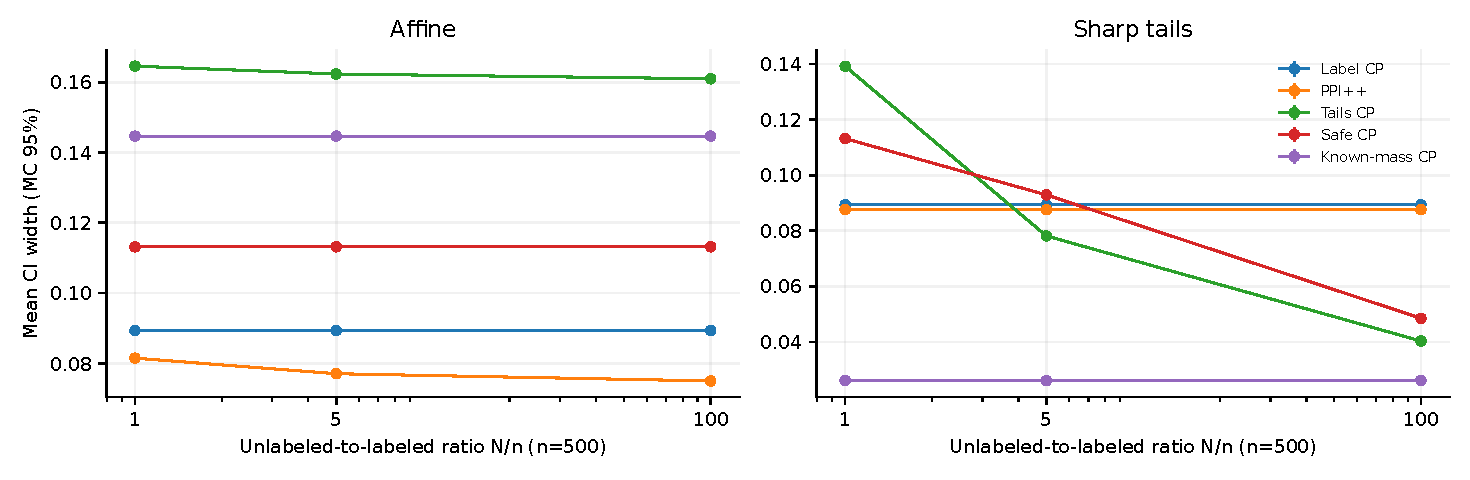
\includegraphics[width=\linewidth]{figures/unlabeled_sensitivity.pdf}
\caption{Finite unlabeled-budget sensitivity at 500 labels, with $1.96$ MCSE bars. Known-mass CP is infeasible and in this figure also reallocates the response error budget; its gap is not purely the price of estimating masses.}\label{fig:sensitivity}
\end{figure}
\begin{table}[h]
\centering\small
\caption{Exploratory post-audit sharp-tail ablation on the same paired inputs. ``Matched'' holds response error $\alpha/(2K)$ fixed; ``reallocated'' uses $\alpha/K$. Mass gap is unknown minus matched-known width; MCSE uses paired differences. True masses are supplied only to the infeasible diagnostics.}\label{tab:mass}
\begin{tabular}{rrrrrr}
\toprule $N/n$ & Unknown weights & Known (matched) & Known (reallocated) & Mass gap & MC SE \\\midrule
1 & 0.1392 & 0.0294 & 0.0262 & 0.1098 & $2.0\times 10^{-5}$ \\
5 & 0.0781 & 0.0293 & 0.0261 & 0.0488 & $8.3\times 10^{-6}$ \\
20 & 0.0538 & 0.0295 & 0.0262 & 0.0243 & $3.0\times 10^{-6}$ \\
100 & 0.0403 & 0.0295 & 0.0262 & 0.0109 & $1.9\times 10^{-6}$ \\
\bottomrule\end{tabular}
\end{table}
The matched-known procedure covers in every observed ablation repetition, but this does not establish true coverage one. The four mass gaps decrease as $N$ increases while the extra response-budget reallocation gap stays near $.00327$. This separates a statistical information effect from a bookkeeping change. The ablation was added after the independent audit noticed the confounding, and is not retroactively included in the locked confirmatory tests.

\begin{figure}[h]
\centering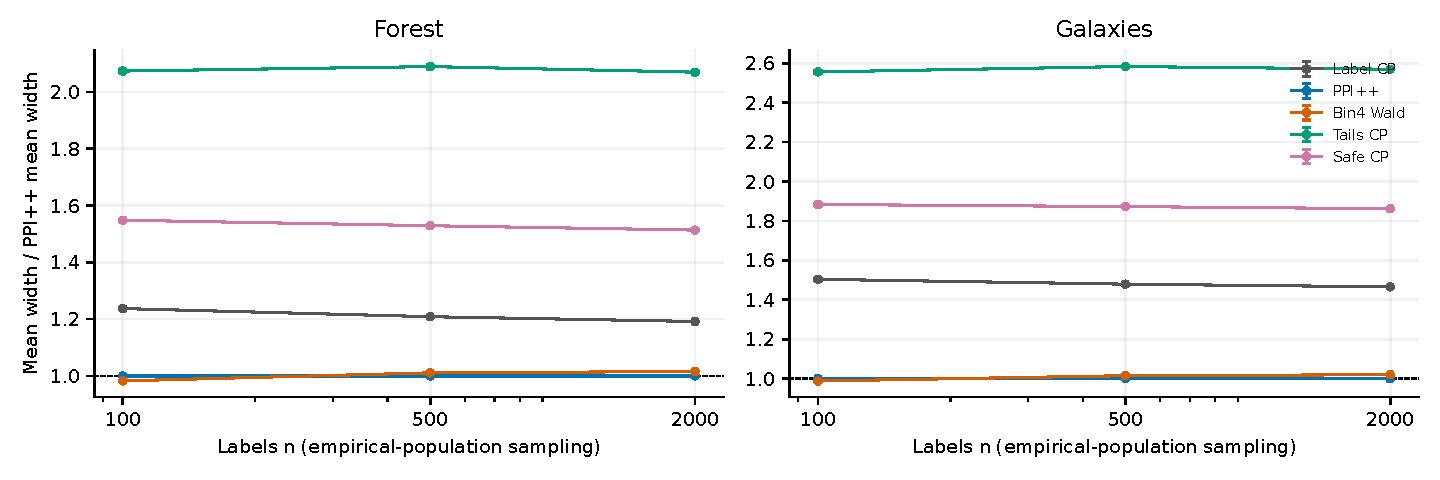
\includegraphics[width=\linewidth]{figures/real_width.pdf}
\caption{Negative real-pool result: width relative to PPI++ under empirical-population resampling. Bars are paired pointwise MC95 ratio intervals from \texttt{paired.csv}; they can be visually small. Marginal width uncertainty and coverage intervals are in Appendix~\ref{app:allresults}. This does not certify finite-sample validity of PPI++.}\label{fig:real}
\end{figure}
\begin{figure}[h]
\centering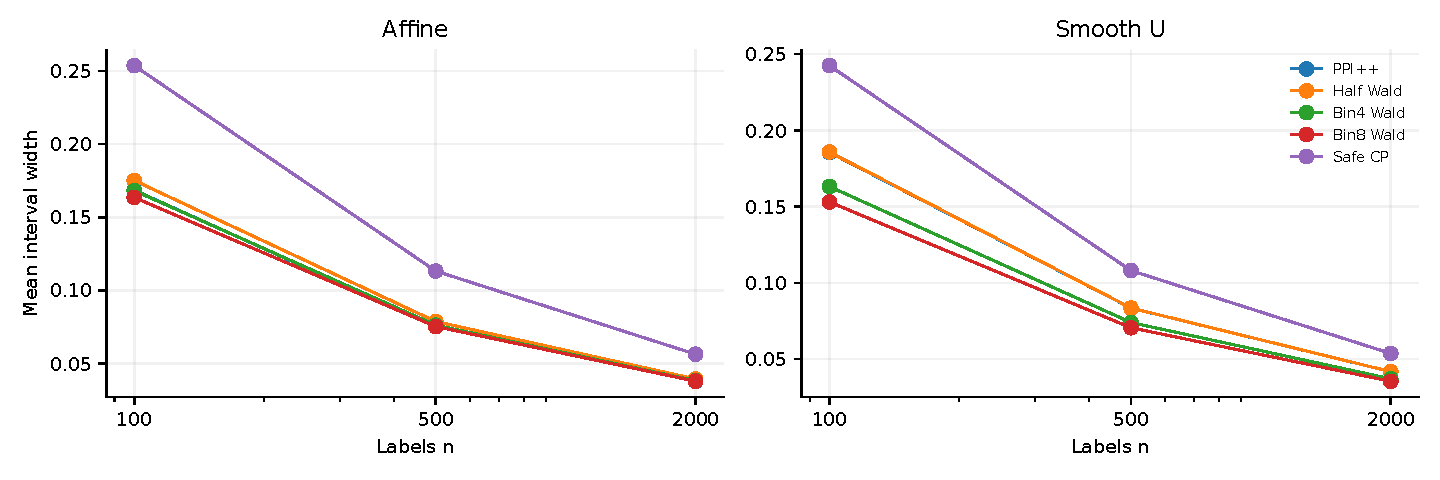
\includegraphics[width=\linewidth]{figures/bin_ablation.pdf}
\caption{Fixed-bin complexity sensitivity. Refinement helps oracle approximation, not necessarily estimated finite-sample widths or coverage. Eight-bin Wald undercoverage at small sample sizes is retained in the full table.}\label{fig:bins}
\end{figure}

\section{Failure log, independence restrictions, and audit scope}\label{app:log}
The initial source-reading agent could not find \texttt{pdftotext}; permitted PDFs downloaded successfully but local extraction failed. A PDF tool then unexpectedly exposed the full permitted PPI++ and Stratified-PPI documents including their bibliographies despite page-limit arguments. Reading stopped as a precaution; no referenced URL was followed and no prohibited identity or confirmed prohibited exposure was recognized. Subsequently \texttt{pypdf} physically restricted extraction to permitted main-text pages before inspection. \texttt{retrieval\_log.md} and \texttt{source\_verification.md} document the exact boundaries. Only the three cited user-allowlisted originals were read; no search engines, citation graphs, paper aggregators, or attempts to identify the excluded paper were used. Official conference style, handbook, checklist and ethics pages were consulted solely for formatting/compliance. A separately attempted system resource query was blocked, and CPU information was obtained using \texttt{lscpu}; this did not affect experiments.

The first analysis command generated summaries and figures but failed in final EDA because of a missing \texttt{counts8} import. Adding the import and rerunning completed it; no observations or numerical method were changed. An initial one-line source extraction command had an unmatched parenthesis and was corrected. Hoeffding/empirical-Bernstein split calibration and trained nonlinear regressors were considered but not implemented or evaluated: the simpler exact binomial route avoids additional fitted-predictor ambiguities and training-label costs. No experimental results are attributed to abandoned methods. The matched-response-budget mass ablation was actually run; it is not a proposed future experiment masquerading as completed evidence.

An independent theory audit rejected unrestricted bin-count monotonicity, required scaled variance consistency and separate degeneracy treatment, and verified the conditional-count/LP/selection construction. An independent analysis audit checked summary-level formulas and selected raw cells; the primary integrity script verified complete pairing, row counts, endpoints, widths and recomputed coverage across all original and supplemental method outputs. The independent audit did not reread every raw output, and neither audit is formal proof-assistant verification or human peer review. Dataset licenses, special-function rounding, numerical-fallback counts, original training independence and deployment generalization remain expressly unresolved rather than silently certified.

\clearpage
\section{All numerical results}\label{app:allresults}
\begingroup\setlength{\tabcolsep}{4pt}\small
\begin{longtable}{llrrrr}
\caption{All results: mean width $\pm$ Monte Carlo SE, coverage and pointwise Wilson 95\% Monte Carlo interval. Shift is outside assumptions; unsafe selection and known-mass results are diagnostics.}\\
\toprule Cell & Method & Width & Coverage & MC lower & MC upper\\\midrule\endfirsthead
\toprule Cell & Method & Width & Coverage & MC lower & MC upper\\\midrule\endhead
Affine 100/2000 & Bin4 CP & $0.50188\pm 3.6\times 10^{-4}$ & 1.0000 & 0.9987 & 1.0000 \\
Affine 100/2000 & Half CP & $0.34451\pm 2.1\times 10^{-4}$ & 1.0000 & 0.9987 & 1.0000 \\
Affine 100/2000 & Tails CP & $0.36119\pm 5.8\times 10^{-5}$ & 0.9997 & 0.9981 & 0.9999 \\
Affine 100/2000 & Label CP & $0.20243\pm 2.4\times 10^{-5}$ & 0.9660 & 0.9589 & 0.9719 \\
Affine 100/2000 & Label Hoeffding & $0.27162\pm 1.0\times 10^{-18}$ & 0.9933 & 0.9897 & 0.9957 \\
Affine 100/2000 & Label Wald & $0.19602\pm 2.5\times 10^{-5}$ & 0.9460 & 0.9373 & 0.9535 \\
Affine 100/2000 & Known-mass CP & $0.32449\pm 6.4\times 10^{-5}$ & 0.9993 & 0.9976 & 0.9998 \\
Affine 100/2000 & PPI & $0.16965\pm 1.8\times 10^{-4}$ & 0.9563 & 0.9484 & 0.9631 \\
Affine 100/2000 & PPI Hoeffding & $0.65828\pm 0$ & 1.0000 & 0.9987 & 1.0000 \\
Affine 100/2000 & PPI++ & $0.16853\pm 1.6\times 10^{-4}$ & 0.9510 & 0.9427 & 0.9582 \\
Affine 100/2000 & Safe CP & $0.25370\pm 3.0\times 10^{-5}$ & 0.9893 & 0.9850 & 0.9924 \\
Affine 100/2000 & Unsafe selection & $0.20243\pm 2.4\times 10^{-5}$ & 0.9660 & 0.9589 & 0.9719 \\
Affine 100/2000 & Bin8 Wald & $0.16354\pm 1.7\times 10^{-4}$ & 0.9347 & 0.9253 & 0.9430 \\
Affine 100/2000 & Bin4 Wald & $0.16820\pm 1.6\times 10^{-4}$ & 0.9470 & 0.9384 & 0.9545 \\
Affine 100/2000 & Half Wald & $0.17513\pm 1.6\times 10^{-4}$ & 0.9500 & 0.9416 & 0.9572 \\
Affine 100/2000 & Tails Wald & $0.19512\pm 3.5\times 10^{-5}$ & 0.9480 & 0.9395 & 0.9554 \\
Affine 500/10000 & Bin4 CP & $0.23395\pm 7.6\times 10^{-5}$ & 1.0000 & 0.9987 & 1.0000 \\
Affine 500/10000 & Half CP & $0.15493\pm 4.0\times 10^{-5}$ & 1.0000 & 0.9987 & 1.0000 \\
Affine 500/10000 & Tails CP & $0.16146\pm 1.0\times 10^{-5}$ & 0.9993 & 0.9976 & 0.9998 \\
Affine 500/10000 & Label CP & $0.08934\pm 2.3\times 10^{-6}$ & 0.9557 & 0.9477 & 0.9625 \\
Affine 500/10000 & Label Hoeffding & $0.12147\pm 5.1\times 10^{-19}$ & 0.9940 & 0.9905 & 0.9962 \\
Affine 500/10000 & Label Wald & $0.08765\pm 2.3\times 10^{-6}$ & 0.9447 & 0.9359 & 0.9523 \\
Affine 500/10000 & Known-mass CP & $0.14468\pm 5.9\times 10^{-6}$ & 0.9980 & 0.9956 & 0.9991 \\
Affine 500/10000 & PPI & $0.07588\pm 3.5\times 10^{-5}$ & 0.9530 & 0.9448 & 0.9600 \\
Affine 500/10000 & PPI Hoeffding & $0.29439\pm 1.0\times 10^{-18}$ & 1.0000 & 0.9987 & 1.0000 \\
Affine 500/10000 & PPI++ & $0.07549\pm 3.1\times 10^{-5}$ & 0.9520 & 0.9438 & 0.9591 \\
Affine 500/10000 & Safe CP & $0.11317\pm 2.9\times 10^{-6}$ & 0.9900 & 0.9858 & 0.9930 \\
Affine 500/10000 & Unsafe selection & $0.08934\pm 2.3\times 10^{-6}$ & 0.9557 & 0.9477 & 0.9625 \\
Affine 500/10000 & Bin8 Wald & $0.07523\pm 3.2\times 10^{-5}$ & 0.9503 & 0.9420 & 0.9575 \\
Affine 500/10000 & Bin4 Wald & $0.07613\pm 3.1\times 10^{-5}$ & 0.9513 & 0.9430 & 0.9585 \\
Affine 500/10000 & Half Wald & $0.07864\pm 3.1\times 10^{-5}$ & 0.9493 & 0.9409 & 0.9566 \\
Affine 500/10000 & Tails Wald & $0.08757\pm 3.1\times 10^{-6}$ & 0.9463 & 0.9377 & 0.9538 \\
Affine 2000/40000 & Bin4 CP & $0.11678\pm 1.9\times 10^{-5}$ & 1.0000 & 0.9987 & 1.0000 \\
Affine 2000/40000 & Half CP & $0.07701\pm 9.9\times 10^{-6}$ & 0.9997 & 0.9981 & 0.9999 \\
Affine 2000/40000 & Tails CP & $0.08004\pm 2.7\times 10^{-6}$ & 0.9990 & 0.9971 & 0.9997 \\
Affine 2000/40000 & Label CP & $0.04429\pm 2.9\times 10^{-7}$ & 0.9507 & 0.9423 & 0.9579 \\
Affine 2000/40000 & Label Hoeffding & $0.06074\pm 8.2\times 10^{-19}$ & 0.9930 & 0.9893 & 0.9954 \\
Affine 2000/40000 & Label Wald & $0.04383\pm 2.9\times 10^{-7}$ & 0.9467 & 0.9380 & 0.9542 \\
Affine 2000/40000 & Known-mass CP & $0.07175\pm 7.5\times 10^{-7}$ & 0.9970 & 0.9943 & 0.9984 \\
Affine 2000/40000 & PPI & $0.03797\pm 8.8\times 10^{-6}$ & 0.9523 & 0.9441 & 0.9594 \\
Affine 2000/40000 & PPI Hoeffding & $0.14720\pm 5.1\times 10^{-19}$ & 1.0000 & 0.9987 & 1.0000 \\
Affine 2000/40000 & PPI++ & $0.03778\pm 7.7\times 10^{-6}$ & 0.9507 & 0.9423 & 0.9579 \\
Affine 2000/40000 & Safe CP & $0.05629\pm 3.7\times 10^{-7}$ & 0.9883 & 0.9838 & 0.9916 \\
Affine 2000/40000 & Unsafe selection & $0.04429\pm 2.9\times 10^{-7}$ & 0.9507 & 0.9423 & 0.9579 \\
Affine 2000/40000 & Bin8 Wald & $0.03782\pm 7.7\times 10^{-6}$ & 0.9493 & 0.9409 & 0.9566 \\
Affine 2000/40000 & Bin4 Wald & $0.03816\pm 7.8\times 10^{-6}$ & 0.9483 & 0.9398 & 0.9557 \\
Affine 2000/40000 & Half Wald & $0.03937\pm 7.6\times 10^{-6}$ & 0.9467 & 0.9380 & 0.9542 \\
Affine 2000/40000 & Tails Wald & $0.04382\pm 4.0\times 10^{-7}$ & 0.9467 & 0.9380 & 0.9542 \\
Reversed 100/2000 & Bin4 CP & $0.50150\pm 3.5\times 10^{-4}$ & 1.0000 & 0.9987 & 1.0000 \\
Reversed 100/2000 & Half CP & $0.34403\pm 2.0\times 10^{-4}$ & 0.9997 & 0.9981 & 0.9999 \\
Reversed 100/2000 & Tails CP & $0.36128\pm 6.0\times 10^{-5}$ & 1.0000 & 0.9987 & 1.0000 \\
Reversed 100/2000 & Label CP & $0.20245\pm 2.4\times 10^{-5}$ & 0.9697 & 0.9629 & 0.9752 \\
Reversed 100/2000 & Label Hoeffding & $0.27162\pm 1.0\times 10^{-18}$ & 0.9930 & 0.9893 & 0.9954 \\
Reversed 100/2000 & Label Wald & $0.19604\pm 2.5\times 10^{-5}$ & 0.9530 & 0.9448 & 0.9600 \\
Reversed 100/2000 & Known-mass CP & $0.32445\pm 6.4\times 10^{-5}$ & 0.9993 & 0.9976 & 0.9998 \\
Reversed 100/2000 & PPI & $0.27395\pm 1.6\times 10^{-4}$ & 0.9523 & 0.9441 & 0.9594 \\
Reversed 100/2000 & PPI Hoeffding & $0.65803\pm 5.1\times 10^{-5}$ & 1.0000 & 0.9987 & 1.0000 \\
Reversed 100/2000 & PPI++ & $0.16816\pm 1.5\times 10^{-4}$ & 0.9493 & 0.9409 & 0.9566 \\
Reversed 100/2000 & Safe CP & $0.25373\pm 3.0\times 10^{-5}$ & 0.9883 & 0.9838 & 0.9916 \\
Reversed 100/2000 & Unsafe selection & $0.20245\pm 2.4\times 10^{-5}$ & 0.9697 & 0.9629 & 0.9752 \\
Reversed 100/2000 & Bin8 Wald & $0.16329\pm 1.6\times 10^{-4}$ & 0.9343 & 0.9249 & 0.9427 \\
Reversed 100/2000 & Bin4 Wald & $0.16786\pm 1.6\times 10^{-4}$ & 0.9427 & 0.9338 & 0.9504 \\
Reversed 100/2000 & Half Wald & $0.17473\pm 1.5\times 10^{-4}$ & 0.9470 & 0.9384 & 0.9545 \\
Reversed 100/2000 & Tails Wald & $0.19509\pm 3.5\times 10^{-5}$ & 0.9523 & 0.9441 & 0.9594 \\
Reversed 500/10000 & Bin4 CP & $0.23383\pm 7.7\times 10^{-5}$ & 1.0000 & 0.9987 & 1.0000 \\
Reversed 500/10000 & Half CP & $0.15498\pm 4.0\times 10^{-5}$ & 0.9997 & 0.9981 & 0.9999 \\
Reversed 500/10000 & Tails CP & $0.16145\pm 9.8\times 10^{-6}$ & 0.9997 & 0.9981 & 0.9999 \\
Reversed 500/10000 & Label CP & $0.08934\pm 2.2\times 10^{-6}$ & 0.9607 & 0.9531 & 0.9671 \\
Reversed 500/10000 & Label Hoeffding & $0.12147\pm 5.1\times 10^{-19}$ & 0.9957 & 0.9926 & 0.9975 \\
Reversed 500/10000 & Label Wald & $0.08765\pm 2.2\times 10^{-6}$ & 0.9517 & 0.9434 & 0.9588 \\
Reversed 500/10000 & Known-mass CP & $0.14469\pm 5.7\times 10^{-6}$ & 0.9987 & 0.9966 & 0.9995 \\
Reversed 500/10000 & PPI & $0.12238\pm 3.0\times 10^{-5}$ & 0.9580 & 0.9502 & 0.9646 \\
Reversed 500/10000 & PPI Hoeffding & $0.29439\pm 1.0\times 10^{-18}$ & 1.0000 & 0.9987 & 1.0000 \\
Reversed 500/10000 & PPI++ & $0.07550\pm 3.1\times 10^{-5}$ & 0.9437 & 0.9348 & 0.9514 \\
Reversed 500/10000 & Safe CP & $0.11317\pm 2.8\times 10^{-6}$ & 0.9913 & 0.9873 & 0.9941 \\
Reversed 500/10000 & Unsafe selection & $0.08934\pm 2.2\times 10^{-6}$ & 0.9607 & 0.9531 & 0.9671 \\
Reversed 500/10000 & Bin8 Wald & $0.07524\pm 3.1\times 10^{-5}$ & 0.9410 & 0.9320 & 0.9489 \\
Reversed 500/10000 & Bin4 Wald & $0.07613\pm 3.1\times 10^{-5}$ & 0.9403 & 0.9313 & 0.9483 \\
Reversed 500/10000 & Half Wald & $0.07868\pm 3.0\times 10^{-5}$ & 0.9433 & 0.9345 & 0.9511 \\
Reversed 500/10000 & Tails Wald & $0.08757\pm 3.0\times 10^{-6}$ & 0.9530 & 0.9448 & 0.9600 \\
Reversed 2000/40000 & Bin4 CP & $0.11675\pm 1.9\times 10^{-5}$ & 1.0000 & 0.9987 & 1.0000 \\
Reversed 2000/40000 & Half CP & $0.07699\pm 1.0\times 10^{-5}$ & 1.0000 & 0.9987 & 1.0000 \\
Reversed 2000/40000 & Tails CP & $0.08004\pm 2.7\times 10^{-6}$ & 0.9993 & 0.9976 & 0.9998 \\
Reversed 2000/40000 & Label CP & $0.04429\pm 2.8\times 10^{-7}$ & 0.9513 & 0.9430 & 0.9585 \\
Reversed 2000/40000 & Label Hoeffding & $0.06074\pm 7.7\times 10^{-19}$ & 0.9940 & 0.9905 & 0.9962 \\
Reversed 2000/40000 & Label Wald & $0.04383\pm 2.8\times 10^{-7}$ & 0.9453 & 0.9366 & 0.9529 \\
Reversed 2000/40000 & Known-mass CP & $0.07175\pm 7.6\times 10^{-7}$ & 0.9987 & 0.9966 & 0.9995 \\
Reversed 2000/40000 & PPI & $0.06120\pm 7.5\times 10^{-6}$ & 0.9477 & 0.9391 & 0.9551 \\
Reversed 2000/40000 & PPI Hoeffding & $0.14720\pm 5.1\times 10^{-19}$ & 1.0000 & 0.9987 & 1.0000 \\
Reversed 2000/40000 & PPI++ & $0.03776\pm 7.8\times 10^{-6}$ & 0.9473 & 0.9388 & 0.9548 \\
Reversed 2000/40000 & Safe CP & $0.05628\pm 3.6\times 10^{-7}$ & 0.9903 & 0.9862 & 0.9933 \\
Reversed 2000/40000 & Unsafe selection & $0.04429\pm 2.8\times 10^{-7}$ & 0.9513 & 0.9430 & 0.9585 \\
Reversed 2000/40000 & Bin8 Wald & $0.03781\pm 7.8\times 10^{-6}$ & 0.9457 & 0.9370 & 0.9532 \\
Reversed 2000/40000 & Bin4 Wald & $0.03815\pm 7.9\times 10^{-6}$ & 0.9510 & 0.9427 & 0.9582 \\
Reversed 2000/40000 & Half Wald & $0.03936\pm 7.7\times 10^{-6}$ & 0.9490 & 0.9405 & 0.9563 \\
Reversed 2000/40000 & Tails Wald & $0.04382\pm 4.1\times 10^{-7}$ & 0.9470 & 0.9384 & 0.9545 \\
Smooth U 100/2000 & Bin4 CP & $0.48788\pm 3.9\times 10^{-4}$ & 1.0000 & 0.9987 & 1.0000 \\
Smooth U 100/2000 & Half CP & $0.34564\pm 2.0\times 10^{-4}$ & 1.0000 & 0.9987 & 1.0000 \\
Smooth U 100/2000 & Tails CP & $0.32202\pm 3.0\times 10^{-4}$ & 1.0000 & 0.9987 & 1.0000 \\
Smooth U 100/2000 & Label CP & $0.19352\pm 1.1\times 10^{-4}$ & 0.9433 & 0.9345 & 0.9511 \\
Smooth U 100/2000 & Label Hoeffding & $0.27162\pm 1.0\times 10^{-18}$ & 0.9943 & 0.9909 & 0.9965 \\
Smooth U 100/2000 & Label Wald & $0.18684\pm 1.2\times 10^{-4}$ & 0.9283 & 0.9185 & 0.9370 \\
Smooth U 100/2000 & Known-mass CP & $0.27163\pm 3.1\times 10^{-4}$ & 0.9993 & 0.9976 & 0.9998 \\
Smooth U 100/2000 & PPI & $0.21920\pm 2.5\times 10^{-4}$ & 0.9377 & 0.9284 & 0.9458 \\
Smooth U 100/2000 & PPI Hoeffding & $0.64389\pm 4.8\times 10^{-4}$ & 1.0000 & 0.9987 & 1.0000 \\
Smooth U 100/2000 & PPI++ & $0.18560\pm 1.2\times 10^{-4}$ & 0.9277 & 0.9178 & 0.9364 \\
Smooth U 100/2000 & Safe CP & $0.24248\pm 1.4\times 10^{-4}$ & 0.9877 & 0.9830 & 0.9910 \\
Smooth U 100/2000 & Unsafe selection & $0.19352\pm 1.1\times 10^{-4}$ & 0.9433 & 0.9345 & 0.9511 \\
Smooth U 100/2000 & Bin8 Wald & $0.15308\pm 1.9\times 10^{-4}$ & 0.9193 & 0.9090 & 0.9286 \\
Smooth U 100/2000 & Bin4 Wald & $0.16318\pm 1.7\times 10^{-4}$ & 0.9297 & 0.9200 & 0.9383 \\
Smooth U 100/2000 & Half Wald & $0.18589\pm 1.2\times 10^{-4}$ & 0.9300 & 0.9203 & 0.9386 \\
Smooth U 100/2000 & Tails Wald & $0.16478\pm 1.7\times 10^{-4}$ & 0.9343 & 0.9249 & 0.9427 \\
Smooth U 500/10000 & Bin4 CP & $0.22649\pm 9.0\times 10^{-5}$ & 1.0000 & 0.9987 & 1.0000 \\
Smooth U 500/10000 & Half CP & $0.15425\pm 3.9\times 10^{-5}$ & 1.0000 & 0.9987 & 1.0000 \\
Smooth U 500/10000 & Tails CP & $0.14438\pm 6.0\times 10^{-5}$ & 0.9997 & 0.9981 & 0.9999 \\
Smooth U 500/10000 & Label CP & $0.08533\pm 2.1\times 10^{-5}$ & 0.9583 & 0.9506 & 0.9649 \\
Smooth U 500/10000 & Label Hoeffding & $0.12147\pm 5.1\times 10^{-19}$ & 0.9967 & 0.9939 & 0.9982 \\
Smooth U 500/10000 & Label Wald & $0.08362\pm 2.2\times 10^{-5}$ & 0.9517 & 0.9434 & 0.9588 \\
Smooth U 500/10000 & Known-mass CP & $0.12016\pm 6.4\times 10^{-5}$ & 0.9990 & 0.9971 & 0.9997 \\
Smooth U 500/10000 & PPI & $0.09835\pm 4.8\times 10^{-5}$ & 0.9457 & 0.9370 & 0.9532 \\
Smooth U 500/10000 & PPI Hoeffding & $0.29439\pm 1.0\times 10^{-18}$ & 1.0000 & 0.9987 & 1.0000 \\
Smooth U 500/10000 & PPI++ & $0.08351\pm 2.2\times 10^{-5}$ & 0.9497 & 0.9413 & 0.9569 \\
Smooth U 500/10000 & Safe CP & $0.10807\pm 2.7\times 10^{-5}$ & 0.9910 & 0.9869 & 0.9938 \\
Smooth U 500/10000 & Unsafe selection & $0.08533\pm 2.1\times 10^{-5}$ & 0.9583 & 0.9506 & 0.9649 \\
Smooth U 500/10000 & Bin8 Wald & $0.07059\pm 3.6\times 10^{-5}$ & 0.9493 & 0.9409 & 0.9566 \\
Smooth U 500/10000 & Bin4 Wald & $0.07402\pm 3.2\times 10^{-5}$ & 0.9483 & 0.9398 & 0.9557 \\
Smooth U 500/10000 & Half Wald & $0.08353\pm 2.2\times 10^{-5}$ & 0.9510 & 0.9427 & 0.9582 \\
Smooth U 500/10000 & Tails Wald & $0.07416\pm 3.2\times 10^{-5}$ & 0.9477 & 0.9391 & 0.9551 \\
Smooth U 2000/40000 & Bin4 CP & $0.11300\pm 2.2\times 10^{-5}$ & 1.0000 & 0.9987 & 1.0000 \\
Smooth U 2000/40000 & Half CP & $0.07638\pm 1.0\times 10^{-5}$ & 1.0000 & 0.9987 & 1.0000 \\
Smooth U 2000/40000 & Tails CP & $0.07166\pm 1.5\times 10^{-5}$ & 1.0000 & 0.9987 & 1.0000 \\
Smooth U 2000/40000 & Label CP & $0.04226\pm 5.4\times 10^{-6}$ & 0.9527 & 0.9445 & 0.9597 \\
Smooth U 2000/40000 & Label Hoeffding & $0.06074\pm 2.5\times 10^{-19}$ & 0.9947 & 0.9914 & 0.9967 \\
Smooth U 2000/40000 & Label Wald & $0.04180\pm 5.4\times 10^{-6}$ & 0.9487 & 0.9402 & 0.9560 \\
Smooth U 2000/40000 & Known-mass CP & $0.05941\pm 1.5\times 10^{-5}$ & 1.0000 & 0.9987 & 1.0000 \\
Smooth U 2000/40000 & PPI & $0.04919\pm 1.2\times 10^{-5}$ & 0.9560 & 0.9481 & 0.9628 \\
Smooth U 2000/40000 & PPI Hoeffding & $0.14720\pm 5.1\times 10^{-19}$ & 1.0000 & 0.9987 & 1.0000 \\
Smooth U 2000/40000 & PPI++ & $0.04178\pm 5.4\times 10^{-6}$ & 0.9477 & 0.9391 & 0.9551 \\
Smooth U 2000/40000 & Safe CP & $0.05371\pm 6.9\times 10^{-6}$ & 0.9900 & 0.9858 & 0.9930 \\
Smooth U 2000/40000 & Unsafe selection & $0.04226\pm 5.4\times 10^{-6}$ & 0.9527 & 0.9445 & 0.9597 \\
Smooth U 2000/40000 & Bin8 Wald & $0.03547\pm 9.1\times 10^{-6}$ & 0.9477 & 0.9391 & 0.9551 \\
Smooth U 2000/40000 & Bin4 Wald & $0.03709\pm 7.9\times 10^{-6}$ & 0.9480 & 0.9395 & 0.9554 \\
Smooth U 2000/40000 & Half Wald & $0.04179\pm 5.4\times 10^{-6}$ & 0.9483 & 0.9398 & 0.9557 \\
Smooth U 2000/40000 & Tails Wald & $0.03711\pm 7.9\times 10^{-6}$ & 0.9480 & 0.9395 & 0.9554 \\
Sharp tails 100/2000 & Bin4 CP & $0.30113\pm 2.2\times 10^{-4}$ & 1.0000 & 0.9987 & 1.0000 \\
Sharp tails 100/2000 & Half CP & $0.36108\pm 6.3\times 10^{-5}$ & 0.9997 & 0.9981 & 0.9999 \\
Sharp tails 100/2000 & Tails CP & $0.15707\pm 2.3\times 10^{-4}$ & 1.0000 & 0.9987 & 1.0000 \\
Sharp tails 100/2000 & Label CP & $0.20237\pm 2.6\times 10^{-5}$ & 0.9620 & 0.9545 & 0.9683 \\
Sharp tails 100/2000 & Label Hoeffding & $0.27162\pm 1.0\times 10^{-18}$ & 0.9913 & 0.9873 & 0.9941 \\
Sharp tails 100/2000 & Label Wald & $0.19597\pm 2.7\times 10^{-5}$ & 0.9413 & 0.9323 & 0.9492 \\
Sharp tails 100/2000 & Known-mass CP & $0.09370\pm 2.3\times 10^{-4}$ & 1.0000 & 0.9987 & 1.0000 \\
Sharp tails 100/2000 & PPI & $0.22756\pm 1.8\times 10^{-4}$ & 0.9437 & 0.9348 & 0.9514 \\
Sharp tails 100/2000 & PPI Hoeffding & $0.65822\pm 3.0\times 10^{-5}$ & 1.0000 & 0.9987 & 1.0000 \\
Sharp tails 100/2000 & PPI++ & $0.19505\pm 3.6\times 10^{-5}$ & 0.9403 & 0.9313 & 0.9483 \\
Sharp tails 100/2000 & Safe CP & $0.18995\pm 2.4\times 10^{-4}$ & 0.9990 & 0.9971 & 0.9997 \\
Sharp tails 100/2000 & Unsafe selection & $0.15702\pm 2.2\times 10^{-4}$ & 0.9977 & 0.9952 & 0.9989 \\
Sharp tails 100/2000 & Bin8 Wald & $0.04926\pm 1.6\times 10^{-4}$ & 0.9473 & 0.9388 & 0.9548 \\
Sharp tails 100/2000 & Bin4 Wald & $0.04950\pm 1.7\times 10^{-4}$ & 0.9490 & 0.9405 & 0.9563 \\
Sharp tails 100/2000 & Half Wald & $0.19506\pm 3.5\times 10^{-5}$ & 0.9407 & 0.9316 & 0.9486 \\
Sharp tails 100/2000 & Tails Wald & $0.04962\pm 1.7\times 10^{-4}$ & 0.9497 & 0.9413 & 0.9569 \\
Sharp tails 500/10000 & Bin4 CP & $0.09987\pm 1.1\times 10^{-4}$ & 1.0000 & 0.9987 & 1.0000 \\
Sharp tails 500/10000 & Half CP & $0.16147\pm 9.9\times 10^{-6}$ & 0.9997 & 0.9981 & 0.9999 \\
Sharp tails 500/10000 & Tails CP & $0.05379\pm 9.4\times 10^{-5}$ & 1.0000 & 0.9987 & 1.0000 \\
Sharp tails 500/10000 & Label CP & $0.08934\pm 2.3\times 10^{-6}$ & 0.9577 & 0.9499 & 0.9643 \\
Sharp tails 500/10000 & Label Hoeffding & $0.12147\pm 5.1\times 10^{-19}$ & 0.9930 & 0.9893 & 0.9954 \\
Sharp tails 500/10000 & Label Wald & $0.08765\pm 2.3\times 10^{-6}$ & 0.9490 & 0.9405 & 0.9563 \\
Sharp tails 500/10000 & Known-mass CP & $0.02621\pm 9.1\times 10^{-5}$ & 1.0000 & 0.9987 & 1.0000 \\
Sharp tails 500/10000 & PPI & $0.10184\pm 3.7\times 10^{-5}$ & 0.9527 & 0.9445 & 0.9597 \\
Sharp tails 500/10000 & PPI Hoeffding & $0.29439\pm 1.0\times 10^{-18}$ & 1.0000 & 0.9987 & 1.0000 \\
Sharp tails 500/10000 & PPI++ & $0.08757\pm 3.1\times 10^{-6}$ & 0.9523 & 0.9441 & 0.9594 \\
Sharp tails 500/10000 & Safe CP & $0.06435\pm 1.0\times 10^{-4}$ & 1.0000 & 0.9987 & 1.0000 \\
Sharp tails 500/10000 & Unsafe selection & $0.05379\pm 9.4\times 10^{-5}$ & 1.0000 & 0.9987 & 1.0000 \\
Sharp tails 500/10000 & Bin8 Wald & $0.02254\pm 3.6\times 10^{-5}$ & 0.9487 & 0.9402 & 0.9560 \\
Sharp tails 500/10000 & Bin4 Wald & $0.02256\pm 3.7\times 10^{-5}$ & 0.9490 & 0.9405 & 0.9563 \\
Sharp tails 500/10000 & Half Wald & $0.08757\pm 3.2\times 10^{-6}$ & 0.9513 & 0.9430 & 0.9585 \\
Sharp tails 500/10000 & Tails Wald & $0.02258\pm 3.7\times 10^{-5}$ & 0.9510 & 0.9427 & 0.9582 \\
Sharp tails 2000/40000 & Bin4 CP & $0.04349\pm 4.2\times 10^{-5}$ & 1.0000 & 0.9987 & 1.0000 \\
Sharp tails 2000/40000 & Half CP & $0.08004\pm 2.7\times 10^{-6}$ & 0.9990 & 0.9971 & 0.9997 \\
Sharp tails 2000/40000 & Tails CP & $0.02467\pm 3.1\times 10^{-5}$ & 1.0000 & 0.9987 & 1.0000 \\
Sharp tails 2000/40000 & Label CP & $0.04429\pm 2.9\times 10^{-7}$ & 0.9500 & 0.9416 & 0.9572 \\
Sharp tails 2000/40000 & Label Hoeffding & $0.06074\pm 7.9\times 10^{-19}$ & 0.9933 & 0.9897 & 0.9957 \\
Sharp tails 2000/40000 & Label Wald & $0.04383\pm 3.0\times 10^{-7}$ & 0.9433 & 0.9345 & 0.9511 \\
Sharp tails 2000/40000 & Known-mass CP & $0.01110\pm 2.8\times 10^{-5}$ & 1.0000 & 0.9987 & 1.0000 \\
Sharp tails 2000/40000 & PPI & $0.05092\pm 9.3\times 10^{-6}$ & 0.9497 & 0.9413 & 0.9569 \\
Sharp tails 2000/40000 & PPI Hoeffding & $0.14720\pm 5.1\times 10^{-19}$ & 1.0000 & 0.9987 & 1.0000 \\
Sharp tails 2000/40000 & PPI++ & $0.04382\pm 4.1\times 10^{-7}$ & 0.9440 & 0.9352 & 0.9517 \\
Sharp tails 2000/40000 & Safe CP & $0.02917\pm 3.5\times 10^{-5}$ & 1.0000 & 0.9987 & 1.0000 \\
Sharp tails 2000/40000 & Unsafe selection & $0.02467\pm 3.1\times 10^{-5}$ & 1.0000 & 0.9987 & 1.0000 \\
Sharp tails 2000/40000 & Bin8 Wald & $0.01128\pm 9.2\times 10^{-6}$ & 0.9553 & 0.9473 & 0.9622 \\
Sharp tails 2000/40000 & Bin4 Wald & $0.01128\pm 9.2\times 10^{-6}$ & 0.9563 & 0.9484 & 0.9631 \\
Sharp tails 2000/40000 & Half Wald & $0.04382\pm 4.0\times 10^{-7}$ & 0.9460 & 0.9373 & 0.9535 \\
Sharp tails 2000/40000 & Tails Wald & $0.01129\pm 9.2\times 10^{-6}$ & 0.9563 & 0.9484 & 0.9631 \\
Irrelevant 100/2000 & Bin4 CP & $0.52007\pm 3.0\times 10^{-4}$ & 1.0000 & 0.9987 & 1.0000 \\
Irrelevant 100/2000 & Half CP & $0.34563\pm 2.0\times 10^{-4}$ & 0.9997 & 0.9981 & 0.9999 \\
Irrelevant 100/2000 & Tails CP & $0.34565\pm 2.0\times 10^{-4}$ & 1.0000 & 0.9987 & 1.0000 \\
Irrelevant 100/2000 & Label CP & $0.19354\pm 1.1\times 10^{-4}$ & 0.9557 & 0.9477 & 0.9625 \\
Irrelevant 100/2000 & Label Hoeffding & $0.27162\pm 1.0\times 10^{-18}$ & 0.9937 & 0.9901 & 0.9959 \\
Irrelevant 100/2000 & Label Wald & $0.18686\pm 1.1\times 10^{-4}$ & 0.9443 & 0.9355 & 0.9520 \\
Irrelevant 100/2000 & Known-mass CP & $0.31041\pm 1.8\times 10^{-4}$ & 0.9983 & 0.9961 & 0.9993 \\
Irrelevant 100/2000 & PPI & $0.21916\pm 2.1\times 10^{-4}$ & 0.9507 & 0.9423 & 0.9579 \\
Irrelevant 100/2000 & PPI Hoeffding & $0.64511\pm 4.5\times 10^{-4}$ & 1.0000 & 0.9987 & 1.0000 \\
Irrelevant 100/2000 & PPI++ & $0.18595\pm 1.1\times 10^{-4}$ & 0.9440 & 0.9352 & 0.9517 \\
Irrelevant 100/2000 & Safe CP & $0.24251\pm 1.4\times 10^{-4}$ & 0.9890 & 0.9846 & 0.9922 \\
Irrelevant 100/2000 & Unsafe selection & $0.19354\pm 1.1\times 10^{-4}$ & 0.9557 & 0.9477 & 0.9625 \\
Irrelevant 100/2000 & Bin8 Wald & $0.18039\pm 1.3\times 10^{-4}$ & 0.9313 & 0.9217 & 0.9398 \\
Irrelevant 100/2000 & Bin4 Wald & $0.18407\pm 1.2\times 10^{-4}$ & 0.9390 & 0.9299 & 0.9470 \\
Irrelevant 100/2000 & Half Wald & $0.18594\pm 1.1\times 10^{-4}$ & 0.9447 & 0.9359 & 0.9523 \\
Irrelevant 100/2000 & Tails Wald & $0.18593\pm 1.1\times 10^{-4}$ & 0.9443 & 0.9355 & 0.9520 \\
Irrelevant 500/10000 & Bin4 CP & $0.23925\pm 6.1\times 10^{-5}$ & 1.0000 & 0.9987 & 1.0000 \\
Irrelevant 500/10000 & Half CP & $0.15416\pm 4.0\times 10^{-5}$ & 0.9997 & 0.9981 & 0.9999 \\
Irrelevant 500/10000 & Tails CP & $0.15416\pm 4.0\times 10^{-5}$ & 0.9997 & 0.9981 & 0.9999 \\
Irrelevant 500/10000 & Label CP & $0.08528\pm 2.2\times 10^{-5}$ & 0.9590 & 0.9513 & 0.9655 \\
Irrelevant 500/10000 & Label Hoeffding & $0.12147\pm 5.1\times 10^{-19}$ & 0.9967 & 0.9939 & 0.9982 \\
Irrelevant 500/10000 & Label Wald & $0.08357\pm 2.2\times 10^{-5}$ & 0.9530 & 0.9448 & 0.9600 \\
Irrelevant 500/10000 & Known-mass CP & $0.13814\pm 3.5\times 10^{-5}$ & 0.9983 & 0.9961 & 0.9993 \\
Irrelevant 500/10000 & PPI & $0.09831\pm 4.1\times 10^{-5}$ & 0.9493 & 0.9409 & 0.9566 \\
Irrelevant 500/10000 & PPI Hoeffding & $0.29439\pm 1.0\times 10^{-18}$ & 1.0000 & 0.9987 & 1.0000 \\
Irrelevant 500/10000 & PPI++ & $0.08348\pm 2.2\times 10^{-5}$ & 0.9527 & 0.9445 & 0.9597 \\
Irrelevant 500/10000 & Safe CP & $0.10800\pm 2.7\times 10^{-5}$ & 0.9900 & 0.9858 & 0.9930 \\
Irrelevant 500/10000 & Unsafe selection & $0.08528\pm 2.2\times 10^{-5}$ & 0.9590 & 0.9513 & 0.9655 \\
Irrelevant 500/10000 & Bin8 Wald & $0.08301\pm 2.2\times 10^{-5}$ & 0.9483 & 0.9398 & 0.9557 \\
Irrelevant 500/10000 & Bin4 Wald & $0.08332\pm 2.2\times 10^{-5}$ & 0.9510 & 0.9427 & 0.9582 \\
Irrelevant 500/10000 & Half Wald & $0.08348\pm 2.2\times 10^{-5}$ & 0.9527 & 0.9445 & 0.9597 \\
Irrelevant 500/10000 & Tails Wald & $0.08348\pm 2.2\times 10^{-5}$ & 0.9517 & 0.9434 & 0.9588 \\
Irrelevant 2000/40000 & Bin4 CP & $0.11875\pm 1.6\times 10^{-5}$ & 1.0000 & 0.9987 & 1.0000 \\
Irrelevant 2000/40000 & Half CP & $0.07639\pm 1.0\times 10^{-5}$ & 0.9997 & 0.9981 & 0.9999 \\
Irrelevant 2000/40000 & Tails CP & $0.07639\pm 1.0\times 10^{-5}$ & 0.9997 & 0.9981 & 0.9999 \\
Irrelevant 2000/40000 & Label CP & $0.04227\pm 5.4\times 10^{-6}$ & 0.9560 & 0.9481 & 0.9628 \\
Irrelevant 2000/40000 & Label Hoeffding & $0.06074\pm 2.5\times 10^{-19}$ & 0.9960 & 0.9930 & 0.9977 \\
Irrelevant 2000/40000 & Label Wald & $0.04180\pm 5.4\times 10^{-6}$ & 0.9523 & 0.9441 & 0.9594 \\
Irrelevant 2000/40000 & Known-mass CP & $0.06848\pm 8.7\times 10^{-6}$ & 0.9987 & 0.9966 & 0.9995 \\
Irrelevant 2000/40000 & PPI & $0.04921\pm 1.0\times 10^{-5}$ & 0.9523 & 0.9441 & 0.9594 \\
Irrelevant 2000/40000 & PPI Hoeffding & $0.14720\pm 5.1\times 10^{-19}$ & 1.0000 & 0.9987 & 1.0000 \\
Irrelevant 2000/40000 & PPI++ & $0.04179\pm 5.4\times 10^{-6}$ & 0.9500 & 0.9416 & 0.9572 \\
Irrelevant 2000/40000 & Safe CP & $0.05371\pm 6.9\times 10^{-6}$ & 0.9870 & 0.9823 & 0.9905 \\
Irrelevant 2000/40000 & Unsafe selection & $0.04227\pm 5.4\times 10^{-6}$ & 0.9560 & 0.9481 & 0.9628 \\
Irrelevant 2000/40000 & Bin8 Wald & $0.04173\pm 5.4\times 10^{-6}$ & 0.9497 & 0.9413 & 0.9569 \\
Irrelevant 2000/40000 & Bin4 Wald & $0.04177\pm 5.4\times 10^{-6}$ & 0.9490 & 0.9405 & 0.9563 \\
Irrelevant 2000/40000 & Half Wald & $0.04179\pm 5.4\times 10^{-6}$ & 0.9497 & 0.9413 & 0.9569 \\
Irrelevant 2000/40000 & Tails Wald & $0.04179\pm 5.4\times 10^{-6}$ & 0.9510 & 0.9427 & 0.9582 \\
Constant 100/2000 & Bin4 CP & $0.26581\pm 1.5\times 10^{-4}$ & 0.9973 & 0.9947 & 0.9986 \\
Constant 100/2000 & Half CP & $0.24436\pm 1.4\times 10^{-4}$ & 0.9943 & 0.9909 & 0.9965 \\
Constant 100/2000 & Tails CP & $0.24436\pm 1.4\times 10^{-4}$ & 0.9943 & 0.9909 & 0.9965 \\
Constant 100/2000 & Label CP & $0.19348\pm 1.1\times 10^{-4}$ & 0.9547 & 0.9466 & 0.9615 \\
Constant 100/2000 & Label Hoeffding & $0.27162\pm 1.0\times 10^{-18}$ & 0.9973 & 0.9947 & 0.9986 \\
Constant 100/2000 & Label Wald & $0.18680\pm 1.1\times 10^{-4}$ & 0.9420 & 0.9331 & 0.9498 \\
Constant 100/2000 & Known-mass CP & $0.21921\pm 1.2\times 10^{-4}$ & 0.9810 & 0.9755 & 0.9853 \\
Constant 100/2000 & PPI & $0.18680\pm 1.1\times 10^{-4}$ & 0.9420 & 0.9331 & 0.9498 \\
Constant 100/2000 & PPI Hoeffding & $0.64800\pm 3.7\times 10^{-4}$ & 1.0000 & 0.9987 & 1.0000 \\
Constant 100/2000 & PPI++ & $0.18680\pm 1.1\times 10^{-4}$ & 0.9420 & 0.9331 & 0.9498 \\
Constant 100/2000 & Safe CP & $0.24244\pm 1.4\times 10^{-4}$ & 0.9943 & 0.9909 & 0.9965 \\
Constant 100/2000 & Unsafe selection & $0.19348\pm 1.1\times 10^{-4}$ & 0.9547 & 0.9466 & 0.9615 \\
Constant 100/2000 & Bin8 Wald & $0.18680\pm 1.1\times 10^{-4}$ & 0.9420 & 0.9331 & 0.9498 \\
Constant 100/2000 & Bin4 Wald & $0.18680\pm 1.1\times 10^{-4}$ & 0.9420 & 0.9331 & 0.9498 \\
Constant 100/2000 & Half Wald & $0.18680\pm 1.1\times 10^{-4}$ & 0.9420 & 0.9331 & 0.9498 \\
Constant 100/2000 & Tails Wald & $0.18680\pm 1.1\times 10^{-4}$ & 0.9420 & 0.9331 & 0.9498 \\
Constant 500/10000 & Bin4 CP & $0.11852\pm 3.0\times 10^{-5}$ & 0.9967 & 0.9939 & 0.9982 \\
Constant 500/10000 & Half CP & $0.10849\pm 2.7\times 10^{-5}$ & 0.9920 & 0.9881 & 0.9946 \\
Constant 500/10000 & Tails CP & $0.10849\pm 2.7\times 10^{-5}$ & 0.9920 & 0.9881 & 0.9946 \\
Constant 500/10000 & Label CP & $0.08530\pm 2.1\times 10^{-5}$ & 0.9580 & 0.9502 & 0.9646 \\
Constant 500/10000 & Label Hoeffding & $0.12147\pm 5.1\times 10^{-19}$ & 0.9970 & 0.9943 & 0.9984 \\
Constant 500/10000 & Label Wald & $0.08359\pm 2.2\times 10^{-5}$ & 0.9520 & 0.9438 & 0.9591 \\
Constant 500/10000 & Known-mass CP & $0.09721\pm 2.4\times 10^{-5}$ & 0.9817 & 0.9762 & 0.9859 \\
Constant 500/10000 & PPI & $0.08359\pm 2.2\times 10^{-5}$ & 0.9520 & 0.9438 & 0.9591 \\
Constant 500/10000 & PPI Hoeffding & $0.29439\pm 1.0\times 10^{-18}$ & 1.0000 & 0.9987 & 1.0000 \\
Constant 500/10000 & PPI++ & $0.08359\pm 2.2\times 10^{-5}$ & 0.9520 & 0.9438 & 0.9591 \\
Constant 500/10000 & Safe CP & $0.10803\pm 2.7\times 10^{-5}$ & 0.9903 & 0.9862 & 0.9933 \\
Constant 500/10000 & Unsafe selection & $0.08530\pm 2.1\times 10^{-5}$ & 0.9580 & 0.9502 & 0.9646 \\
Constant 500/10000 & Bin8 Wald & $0.08359\pm 2.2\times 10^{-5}$ & 0.9520 & 0.9438 & 0.9591 \\
Constant 500/10000 & Bin4 Wald & $0.08359\pm 2.2\times 10^{-5}$ & 0.9520 & 0.9438 & 0.9591 \\
Constant 500/10000 & Half Wald & $0.08359\pm 2.2\times 10^{-5}$ & 0.9520 & 0.9438 & 0.9591 \\
Constant 500/10000 & Tails Wald & $0.08359\pm 2.2\times 10^{-5}$ & 0.9520 & 0.9438 & 0.9591 \\
Constant 2000/40000 & Bin4 CP & $0.05890\pm 7.5\times 10^{-6}$ & 0.9937 & 0.9901 & 0.9959 \\
Constant 2000/40000 & Half CP & $0.05385\pm 6.8\times 10^{-6}$ & 0.9877 & 0.9830 & 0.9910 \\
Constant 2000/40000 & Tails CP & $0.05385\pm 6.8\times 10^{-6}$ & 0.9877 & 0.9830 & 0.9910 \\
Constant 2000/40000 & Label CP & $0.04228\pm 5.3\times 10^{-6}$ & 0.9623 & 0.9549 & 0.9686 \\
Constant 2000/40000 & Label Hoeffding & $0.06074\pm 2.5\times 10^{-19}$ & 0.9943 & 0.9909 & 0.9965 \\
Constant 2000/40000 & Label Wald & $0.04181\pm 5.4\times 10^{-6}$ & 0.9590 & 0.9513 & 0.9655 \\
Constant 2000/40000 & Known-mass CP & $0.04827\pm 6.1\times 10^{-6}$ & 0.9793 & 0.9736 & 0.9838 \\
Constant 2000/40000 & PPI & $0.04181\pm 5.4\times 10^{-6}$ & 0.9590 & 0.9513 & 0.9655 \\
Constant 2000/40000 & PPI Hoeffding & $0.14720\pm 5.1\times 10^{-19}$ & 1.0000 & 0.9987 & 1.0000 \\
Constant 2000/40000 & PPI++ & $0.04181\pm 5.4\times 10^{-6}$ & 0.9590 & 0.9513 & 0.9655 \\
Constant 2000/40000 & Safe CP & $0.05373\pm 6.8\times 10^{-6}$ & 0.9877 & 0.9830 & 0.9910 \\
Constant 2000/40000 & Unsafe selection & $0.04228\pm 5.3\times 10^{-6}$ & 0.9623 & 0.9549 & 0.9686 \\
Constant 2000/40000 & Bin8 Wald & $0.04181\pm 5.4\times 10^{-6}$ & 0.9590 & 0.9513 & 0.9655 \\
Constant 2000/40000 & Bin4 Wald & $0.04181\pm 5.4\times 10^{-6}$ & 0.9590 & 0.9513 & 0.9655 \\
Constant 2000/40000 & Half Wald & $0.04181\pm 5.4\times 10^{-6}$ & 0.9590 & 0.9513 & 0.9655 \\
Constant 2000/40000 & Tails Wald & $0.04181\pm 5.4\times 10^{-6}$ & 0.9590 & 0.9513 & 0.9655 \\
Rare tails 100/2000 & Bin4 CP & $0.23127\pm 3.4\times 10^{-4}$ & 1.0000 & 0.9987 & 1.0000 \\
Rare tails 100/2000 & Half CP & $0.11627\pm 3.3\times 10^{-4}$ & 0.9997 & 0.9981 & 0.9999 \\
Rare tails 100/2000 & Tails CP & $0.11581\pm 3.1\times 10^{-4}$ & 0.9980 & 0.9956 & 0.9991 \\
Rare tails 100/2000 & Label CP & $0.05208\pm 2.6\times 10^{-4}$ & 0.9820 & 0.9766 & 0.9862 \\
Rare tails 100/2000 & Label Hoeffding & $0.14565\pm 1.8\times 10^{-4}$ & 1.0000 & 0.9987 & 1.0000 \\
Rare tails 100/2000 & Label Wald & $0.02469\pm 4.0\times 10^{-4}$ & 0.6263 & 0.6089 & 0.6435 \\
Rare tails 100/2000 & Known-mass CP & $0.10116\pm 2.8\times 10^{-4}$ & 0.9957 & 0.9926 & 0.9975 \\
Rare tails 100/2000 & PPI & $0.06943\pm 5.7\times 10^{-4}$ & 0.9513 & 0.9430 & 0.9585 \\
Rare tails 100/2000 & PPI Hoeffding & $0.33803\pm 5.7\times 10^{-4}$ & 1.0000 & 0.9987 & 1.0000 \\
Rare tails 100/2000 & PPI++ & $0.02449\pm 4.0\times 10^{-4}$ & 0.6260 & 0.6085 & 0.6431 \\
Rare tails 100/2000 & Safe CP & $0.06749\pm 3.1\times 10^{-4}$ & 0.9960 & 0.9930 & 0.9977 \\
Rare tails 100/2000 & Unsafe selection & $0.05208\pm 2.6\times 10^{-4}$ & 0.9820 & 0.9766 & 0.9862 \\
Rare tails 100/2000 & Bin8 Wald & $0.02398\pm 3.9\times 10^{-4}$ & 0.6217 & 0.6042 & 0.6389 \\
Rare tails 100/2000 & Bin4 Wald & $0.02436\pm 3.9\times 10^{-4}$ & 0.6240 & 0.6065 & 0.6412 \\
Rare tails 100/2000 & Half Wald & $0.02461\pm 4.0\times 10^{-4}$ & 0.6260 & 0.6085 & 0.6431 \\
Rare tails 100/2000 & Tails Wald & $0.02456\pm 3.9\times 10^{-4}$ & 0.6253 & 0.6079 & 0.6425 \\
Rare tails 500/10000 & Bin4 CP & $0.06384\pm 1.3\times 10^{-4}$ & 1.0000 & 0.9987 & 1.0000 \\
Rare tails 500/10000 & Half CP & $0.03710\pm 1.2\times 10^{-4}$ & 0.9997 & 0.9981 & 0.9999 \\
Rare tails 500/10000 & Tails CP & $0.03537\pm 9.7\times 10^{-5}$ & 0.9983 & 0.9961 & 0.9993 \\
Rare tails 500/10000 & Label CP & $0.01952\pm 7.2\times 10^{-5}$ & 0.9753 & 0.9691 & 0.9803 \\
Rare tails 500/10000 & Label Hoeffding & $0.07079\pm 8.3\times 10^{-5}$ & 1.0000 & 0.9987 & 1.0000 \\
Rare tails 500/10000 & Label Wald & $0.01665\pm 8.6\times 10^{-5}$ & 0.8647 & 0.8520 & 0.8764 \\
Rare tails 500/10000 & Known-mass CP & $0.03114\pm 8.6\times 10^{-5}$ & 0.9930 & 0.9893 & 0.9954 \\
Rare tails 500/10000 & PPI & $0.03677\pm 2.4\times 10^{-4}$ & 0.9450 & 0.9363 & 0.9526 \\
Rare tails 500/10000 & PPI Hoeffding & $0.15729\pm 2.6\times 10^{-4}$ & 1.0000 & 0.9987 & 1.0000 \\
Rare tails 500/10000 & PPI++ & $0.01662\pm 8.6\times 10^{-5}$ & 0.8660 & 0.8533 & 0.8777 \\
Rare tails 500/10000 & Safe CP & $0.02463\pm 8.9\times 10^{-5}$ & 0.9947 & 0.9914 & 0.9967 \\
Rare tails 500/10000 & Unsafe selection & $0.01952\pm 7.2\times 10^{-5}$ & 0.9753 & 0.9691 & 0.9803 \\
Rare tails 500/10000 & Bin8 Wald & $0.01648\pm 8.4\times 10^{-5}$ & 0.8687 & 0.8561 & 0.8803 \\
Rare tails 500/10000 & Bin4 Wald & $0.01654\pm 8.5\times 10^{-5}$ & 0.8663 & 0.8537 & 0.8780 \\
Rare tails 500/10000 & Half Wald & $0.01664\pm 8.6\times 10^{-5}$ & 0.8647 & 0.8520 & 0.8764 \\
Rare tails 500/10000 & Tails Wald & $0.01658\pm 8.5\times 10^{-5}$ & 0.8657 & 0.8530 & 0.8774 \\
Rare tails 2000/40000 & Bin4 CP & $0.02499\pm 4.0\times 10^{-5}$ & 1.0000 & 0.9987 & 1.0000 \\
Rare tails 2000/40000 & Half CP & $0.01684\pm 3.2\times 10^{-5}$ & 1.0000 & 0.9987 & 1.0000 \\
Rare tails 2000/40000 & Tails CP & $0.01500\pm 2.8\times 10^{-5}$ & 0.9993 & 0.9976 & 0.9998 \\
Rare tails 2000/40000 & Label CP & $0.00920\pm 1.8\times 10^{-5}$ & 0.9527 & 0.9445 & 0.9597 \\
Rare tails 2000/40000 & Label Hoeffding & $0.04031\pm 4.0\times 10^{-5}$ & 1.0000 & 0.9987 & 1.0000 \\
Rare tails 2000/40000 & Label Wald & $0.00864\pm 1.8\times 10^{-5}$ & 0.9453 & 0.9366 & 0.9529 \\
Rare tails 2000/40000 & Known-mass CP & $0.01325\pm 2.5\times 10^{-5}$ & 0.9960 & 0.9930 & 0.9977 \\
Rare tails 2000/40000 & PPI & $0.02228\pm 9.6\times 10^{-5}$ & 0.9547 & 0.9466 & 0.9615 \\
Rare tails 2000/40000 & PPI Hoeffding & $0.08335\pm 1.2\times 10^{-4}$ & 1.0000 & 0.9987 & 1.0000 \\
Rare tails 2000/40000 & PPI++ & $0.00864\pm 1.8\times 10^{-5}$ & 0.9370 & 0.9277 & 0.9451 \\
Rare tails 2000/40000 & Safe CP & $0.01163\pm 2.2\times 10^{-5}$ & 0.9927 & 0.9889 & 0.9952 \\
Rare tails 2000/40000 & Unsafe selection & $0.00920\pm 1.8\times 10^{-5}$ & 0.9527 & 0.9445 & 0.9597 \\
Rare tails 2000/40000 & Bin8 Wald & $0.00860\pm 1.7\times 10^{-5}$ & 0.9353 & 0.9260 & 0.9436 \\
Rare tails 2000/40000 & Bin4 Wald & $0.00860\pm 1.8\times 10^{-5}$ & 0.9353 & 0.9260 & 0.9436 \\
Rare tails 2000/40000 & Half Wald & $0.00864\pm 1.8\times 10^{-5}$ & 0.9410 & 0.9320 & 0.9489 \\
Rare tails 2000/40000 & Tails Wald & $0.00861\pm 1.8\times 10^{-5}$ & 0.9377 & 0.9284 & 0.9458 \\
Shift 100/2000 & Bin4 CP & $0.46289\pm 8.3\times 10^{-4}$ & 0.7167 & 0.7003 & 0.7325 \\
Shift 100/2000 & Half CP & $0.33252\pm 4.3\times 10^{-4}$ & 0.4340 & 0.4164 & 0.4518 \\
Shift 100/2000 & Tails CP & $0.36101\pm 1.4\times 10^{-4}$ & 0.9993 & 0.9976 & 0.9998 \\
Shift 100/2000 & Label CP & $0.20238\pm 2.5\times 10^{-5}$ & 0.9637 & 0.9564 & 0.9698 \\
Shift 100/2000 & Label Hoeffding & $0.27162\pm 1.0\times 10^{-18}$ & 0.9907 & 0.9865 & 0.9935 \\
Shift 100/2000 & Label Wald & $0.19597\pm 2.6\times 10^{-5}$ & 0.9460 & 0.9373 & 0.9535 \\
Shift 100/2000 & Known-mass CP & $0.32441\pm 6.4\times 10^{-5}$ & 0.9993 & 0.9976 & 0.9998 \\
Shift 100/2000 & PPI & $0.16840\pm 1.8\times 10^{-4}$ & 0.0000 & 0.0000 & 0.0013 \\
Shift 100/2000 & PPI Hoeffding & $0.52901\pm 8.0\times 10^{-4}$ & 0.7413 & 0.7254 & 0.7567 \\
Shift 100/2000 & PPI++ & $0.03115\pm 9.6\times 10^{-4}$ & 0.0000 & 0.0000 & 0.0013 \\
Shift 100/2000 & Safe CP & $0.25364\pm 3.2\times 10^{-5}$ & 0.9850 & 0.9800 & 0.9888 \\
Shift 100/2000 & Unsafe selection & $0.20238\pm 2.5\times 10^{-5}$ & 0.9637 & 0.9564 & 0.9698 \\
Shift 100/2000 & Bin8 Wald & $0.16266\pm 1.7\times 10^{-4}$ & 0.0030 & 0.0016 & 0.0057 \\
Shift 100/2000 & Bin4 Wald & $0.16741\pm 1.6\times 10^{-4}$ & 0.0050 & 0.0030 & 0.0082 \\
Shift 100/2000 & Half Wald & $0.17439\pm 1.6\times 10^{-4}$ & 0.0597 & 0.0517 & 0.0687 \\
Shift 100/2000 & Tails Wald & $0.19506\pm 3.5\times 10^{-5}$ & 0.9337 & 0.9242 & 0.9420 \\
Shift 500/10000 & Bin4 CP & $0.21271\pm 1.9\times 10^{-4}$ & 0.0000 & 0.0000 & 0.0013 \\
Shift 500/10000 & Half CP & $0.14937\pm 8.9\times 10^{-5}$ & 0.0000 & 0.0000 & 0.0013 \\
Shift 500/10000 & Tails CP & $0.16142\pm 2.6\times 10^{-5}$ & 0.9990 & 0.9971 & 0.9997 \\
Shift 500/10000 & Label CP & $0.08934\pm 2.4\times 10^{-6}$ & 0.9507 & 0.9423 & 0.9579 \\
Shift 500/10000 & Label Hoeffding & $0.12147\pm 5.1\times 10^{-19}$ & 0.9923 & 0.9885 & 0.9949 \\
Shift 500/10000 & Label Wald & $0.08765\pm 2.4\times 10^{-6}$ & 0.9420 & 0.9331 & 0.9498 \\
Shift 500/10000 & Known-mass CP & $0.14468\pm 5.9\times 10^{-6}$ & 0.9980 & 0.9956 & 0.9991 \\
Shift 500/10000 & PPI & $0.07529\pm 3.6\times 10^{-5}$ & 0.0000 & 0.0000 & 0.0013 \\
Shift 500/10000 & PPI Hoeffding & $0.29438\pm 5.3\times 10^{-6}$ & 0.0000 & 0.0000 & 0.0013 \\
Shift 500/10000 & PPI++ & $0.00078\pm 9.0\times 10^{-5}$ & 0.0000 & 0.0000 & 0.0013 \\
Shift 500/10000 & Safe CP & $0.11317\pm 3.0\times 10^{-6}$ & 0.9893 & 0.9850 & 0.9924 \\
Shift 500/10000 & Unsafe selection & $0.08934\pm 2.4\times 10^{-6}$ & 0.9507 & 0.9423 & 0.9579 \\
Shift 500/10000 & Bin8 Wald & $0.07479\pm 3.3\times 10^{-5}$ & 0.0000 & 0.0000 & 0.0013 \\
Shift 500/10000 & Bin4 Wald & $0.07571\pm 3.3\times 10^{-5}$ & 0.0000 & 0.0000 & 0.0013 \\
Shift 500/10000 & Half Wald & $0.07833\pm 3.3\times 10^{-5}$ & 0.0000 & 0.0000 & 0.0013 \\
Shift 500/10000 & Tails Wald & $0.08757\pm 3.2\times 10^{-6}$ & 0.9273 & 0.9175 & 0.9361 \\
Shift 2000/40000 & Bin4 CP & $0.10591\pm 4.7\times 10^{-5}$ & 0.0000 & 0.0000 & 0.0013 \\
Shift 2000/40000 & Half CP & $0.07413\pm 2.2\times 10^{-5}$ & 0.0000 & 0.0000 & 0.0013 \\
Shift 2000/40000 & Tails CP & $0.08001\pm 6.6\times 10^{-6}$ & 0.9983 & 0.9961 & 0.9993 \\
Shift 2000/40000 & Label CP & $0.04429\pm 2.8\times 10^{-7}$ & 0.9530 & 0.9448 & 0.9600 \\
Shift 2000/40000 & Label Hoeffding & $0.06074\pm 7.8\times 10^{-19}$ & 0.9937 & 0.9901 & 0.9959 \\
Shift 2000/40000 & Label Wald & $0.04383\pm 2.8\times 10^{-7}$ & 0.9483 & 0.9398 & 0.9557 \\
Shift 2000/40000 & Known-mass CP & $0.07175\pm 7.3\times 10^{-7}$ & 0.9977 & 0.9952 & 0.9989 \\
Shift 2000/40000 & PPI & $0.03766\pm 8.9\times 10^{-6}$ & 0.0000 & 0.0000 & 0.0013 \\
Shift 2000/40000 & PPI Hoeffding & $0.14720\pm 5.1\times 10^{-19}$ & 0.0000 & 0.0000 & 0.0013 \\
Shift 2000/40000 & PPI++ & $0.00000\pm 0$ & 0.0000 & 0.0000 & 0.0013 \\
Shift 2000/40000 & Safe CP & $0.05628\pm 3.6\times 10^{-7}$ & 0.9887 & 0.9842 & 0.9919 \\
Shift 2000/40000 & Unsafe selection & $0.04429\pm 2.8\times 10^{-7}$ & 0.9530 & 0.9448 & 0.9600 \\
Shift 2000/40000 & Bin8 Wald & $0.03760\pm 8.1\times 10^{-6}$ & 0.0000 & 0.0000 & 0.0013 \\
Shift 2000/40000 & Bin4 Wald & $0.03794\pm 8.1\times 10^{-6}$ & 0.0000 & 0.0000 & 0.0013 \\
Shift 2000/40000 & Half Wald & $0.03918\pm 7.9\times 10^{-6}$ & 0.0000 & 0.0000 & 0.0013 \\
Shift 2000/40000 & Tails Wald & $0.04382\pm 3.9\times 10^{-7}$ & 0.9347 & 0.9253 & 0.9430 \\
Affine 500/500 & Bin4 CP & $0.30333\pm 1.1\times 10^{-4}$ & 1.0000 & 0.9974 & 1.0000 \\
Affine 500/500 & Half CP & $0.19386\pm 3.4\times 10^{-5}$ & 1.0000 & 0.9974 & 1.0000 \\
Affine 500/500 & Tails CP & $0.16458\pm 7.4\times 10^{-5}$ & 0.9987 & 0.9952 & 0.9996 \\
Affine 500/500 & Label CP & $0.08934\pm 3.5\times 10^{-6}$ & 0.9520 & 0.9400 & 0.9617 \\
Affine 500/500 & Label Hoeffding & $0.12147\pm 7.2\times 10^{-19}$ & 0.9927 & 0.9869 & 0.9959 \\
Affine 500/500 & Label Wald & $0.08765\pm 3.6\times 10^{-6}$ & 0.9420 & 0.9290 & 0.9527 \\
Affine 500/500 & Known-mass CP & $0.14467\pm 8.8\times 10^{-6}$ & 0.9980 & 0.9941 & 0.9993 \\
Affine 500/500 & PPI & $0.09052\pm 4.4\times 10^{-5}$ & 0.9460 & 0.9334 & 0.9563 \\
Affine 500/500 & PPI Hoeffding & $0.39718\pm 2.9\times 10^{-18}$ & 1.0000 & 0.9974 & 1.0000 \\
Affine 500/500 & PPI++ & $0.08149\pm 2.2\times 10^{-5}$ & 0.9493 & 0.9370 & 0.9593 \\
Affine 500/500 & Safe CP & $0.11316\pm 4.5\times 10^{-6}$ & 0.9900 & 0.9836 & 0.9939 \\
Affine 500/500 & Unsafe selection & $0.08934\pm 3.5\times 10^{-6}$ & 0.9520 & 0.9400 & 0.9617 \\
Affine 500/500 & Bin8 Wald & $0.08138\pm 2.3\times 10^{-5}$ & 0.9467 & 0.9341 & 0.9569 \\
Affine 500/500 & Bin4 Wald & $0.08181\pm 2.2\times 10^{-5}$ & 0.9487 & 0.9363 & 0.9587 \\
Affine 500/500 & Half Wald & $0.08304\pm 2.2\times 10^{-5}$ & 0.9513 & 0.9392 & 0.9611 \\
Affine 500/500 & Tails Wald & $0.08760\pm 3.9\times 10^{-6}$ & 0.9447 & 0.9319 & 0.9551 \\
Affine 500/2500 & Bin4 CP & $0.25404\pm 8.5\times 10^{-5}$ & 1.0000 & 0.9974 & 1.0000 \\
Affine 500/2500 & Half CP & $0.16608\pm 3.1\times 10^{-5}$ & 1.0000 & 0.9974 & 1.0000 \\
Affine 500/2500 & Tails CP & $0.16235\pm 2.9\times 10^{-5}$ & 1.0000 & 0.9974 & 1.0000 \\
Affine 500/2500 & Label CP & $0.08934\pm 3.1\times 10^{-6}$ & 0.9607 & 0.9496 & 0.9694 \\
Affine 500/2500 & Label Hoeffding & $0.12147\pm 7.2\times 10^{-19}$ & 0.9940 & 0.9886 & 0.9968 \\
Affine 500/2500 & Label Wald & $0.08765\pm 3.1\times 10^{-6}$ & 0.9460 & 0.9334 & 0.9563 \\
Affine 500/2500 & Known-mass CP & $0.14467\pm 8.1\times 10^{-6}$ & 1.0000 & 0.9974 & 1.0000 \\
Affine 500/2500 & PPI & $0.07832\pm 4.6\times 10^{-5}$ & 0.9560 & 0.9444 & 0.9653 \\
Affine 500/2500 & PPI Hoeffding & $0.32400\pm 1.4\times 10^{-18}$ & 1.0000 & 0.9974 & 1.0000 \\
Affine 500/2500 & PPI++ & $0.07708\pm 3.6\times 10^{-5}$ & 0.9593 & 0.9481 & 0.9682 \\
Affine 500/2500 & Safe CP & $0.11317\pm 3.9\times 10^{-6}$ & 0.9880 & 0.9811 & 0.9924 \\
Affine 500/2500 & Unsafe selection & $0.08934\pm 3.1\times 10^{-6}$ & 0.9607 & 0.9496 & 0.9694 \\
Affine 500/2500 & Bin8 Wald & $0.07687\pm 3.7\times 10^{-5}$ & 0.9580 & 0.9466 & 0.9670 \\
Affine 500/2500 & Bin4 Wald & $0.07764\pm 3.7\times 10^{-5}$ & 0.9567 & 0.9451 & 0.9659 \\
Affine 500/2500 & Half Wald & $0.07982\pm 3.6\times 10^{-5}$ & 0.9547 & 0.9429 & 0.9641 \\
Affine 500/2500 & Tails Wald & $0.08758\pm 4.0\times 10^{-6}$ & 0.9513 & 0.9392 & 0.9611 \\
Affine 500/50000 & Bin4 CP & $0.22278\pm 1.2\times 10^{-4}$ & 1.0000 & 0.9974 & 1.0000 \\
Affine 500/50000 & Half CP & $0.14888\pm 7.1\times 10^{-5}$ & 0.9993 & 0.9962 & 0.9999 \\
Affine 500/50000 & Tails CP & $0.16097\pm 8.1\times 10^{-6}$ & 1.0000 & 0.9974 & 1.0000 \\
Affine 500/50000 & Label CP & $0.08934\pm 3.3\times 10^{-6}$ & 0.9560 & 0.9444 & 0.9653 \\
Affine 500/50000 & Label Hoeffding & $0.12147\pm 7.2\times 10^{-19}$ & 0.9920 & 0.9861 & 0.9954 \\
Affine 500/50000 & Label Wald & $0.08765\pm 3.3\times 10^{-6}$ & 0.9453 & 0.9327 & 0.9557 \\
Affine 500/50000 & Known-mass CP & $0.14468\pm 8.5\times 10^{-6}$ & 0.9980 & 0.9941 & 0.9993 \\
Affine 500/50000 & PPI & $0.07524\pm 5.0\times 10^{-5}$ & 0.9573 & 0.9459 & 0.9664 \\
Affine 500/50000 & PPI Hoeffding & $0.27803\pm 0$ & 1.0000 & 0.9974 & 1.0000 \\
Affine 500/50000 & PPI++ & $0.07500\pm 4.5\times 10^{-5}$ & 0.9547 & 0.9429 & 0.9641 \\
Affine 500/50000 & Safe CP & $0.11317\pm 4.2\times 10^{-6}$ & 0.9867 & 0.9795 & 0.9914 \\
Affine 500/50000 & Unsafe selection & $0.08934\pm 3.3\times 10^{-6}$ & 0.9560 & 0.9444 & 0.9653 \\
Affine 500/50000 & Bin8 Wald & $0.07472\pm 4.5\times 10^{-5}$ & 0.9500 & 0.9378 & 0.9599 \\
Affine 500/50000 & Bin4 Wald & $0.07566\pm 4.5\times 10^{-5}$ & 0.9527 & 0.9407 & 0.9623 \\
Affine 500/50000 & Half Wald & $0.07831\pm 4.5\times 10^{-5}$ & 0.9513 & 0.9392 & 0.9611 \\
Affine 500/50000 & Tails Wald & $0.08757\pm 4.6\times 10^{-6}$ & 0.9493 & 0.9370 & 0.9593 \\
Sharp tails 500/500 & Bin4 CP & $0.24795\pm 1.2\times 10^{-4}$ & 1.0000 & 0.9974 & 1.0000 \\
Sharp tails 500/500 & Half CP & $0.16456\pm 7.3\times 10^{-5}$ & 1.0000 & 0.9974 & 1.0000 \\
Sharp tails 500/500 & Tails CP & $0.13919\pm 1.2\times 10^{-4}$ & 1.0000 & 0.9974 & 1.0000 \\
Sharp tails 500/500 & Label CP & $0.08934\pm 3.2\times 10^{-6}$ & 0.9500 & 0.9378 & 0.9599 \\
Sharp tails 500/500 & Label Hoeffding & $0.12147\pm 7.2\times 10^{-19}$ & 0.9940 & 0.9886 & 0.9968 \\
Sharp tails 500/500 & Label Wald & $0.08765\pm 3.3\times 10^{-6}$ & 0.9373 & 0.9239 & 0.9485 \\
Sharp tails 500/500 & Known-mass CP & $0.02616\pm 1.3\times 10^{-4}$ & 1.0000 & 0.9974 & 1.0000 \\
Sharp tails 500/500 & PPI & $0.11313\pm 4.7\times 10^{-5}$ & 0.9487 & 0.9363 & 0.9587 \\
Sharp tails 500/500 & PPI Hoeffding & $0.39718\pm 2.9\times 10^{-18}$ & 1.0000 & 0.9974 & 1.0000 \\
Sharp tails 500/500 & PPI++ & $0.08761\pm 3.6\times 10^{-6}$ & 0.9407 & 0.9275 & 0.9515 \\
Sharp tails 500/500 & Safe CP & $0.11317\pm 4.1\times 10^{-6}$ & 0.9907 & 0.9844 & 0.9944 \\
Sharp tails 500/500 & Unsafe selection & $0.08934\pm 3.2\times 10^{-6}$ & 0.9500 & 0.9378 & 0.9599 \\
Sharp tails 500/500 & Bin8 Wald & $0.06259\pm 1.0\times 10^{-5}$ & 0.9513 & 0.9392 & 0.9611 \\
Sharp tails 500/500 & Bin4 Wald & $0.06259\pm 1.0\times 10^{-5}$ & 0.9520 & 0.9400 & 0.9617 \\
Sharp tails 500/500 & Half Wald & $0.08761\pm 3.6\times 10^{-6}$ & 0.9387 & 0.9254 & 0.9497 \\
Sharp tails 500/500 & Tails Wald & $0.06260\pm 1.0\times 10^{-5}$ & 0.9527 & 0.9407 & 0.9623 \\
Sharp tails 500/2500 & Bin4 CP & $0.14339\pm 1.4\times 10^{-4}$ & 1.0000 & 0.9974 & 1.0000 \\
Sharp tails 500/2500 & Half CP & $0.16241\pm 3.0\times 10^{-5}$ & 0.9993 & 0.9962 & 0.9999 \\
Sharp tails 500/2500 & Tails CP & $0.07813\pm 1.3\times 10^{-4}$ & 1.0000 & 0.9974 & 1.0000 \\
Sharp tails 500/2500 & Label CP & $0.08934\pm 3.2\times 10^{-6}$ & 0.9593 & 0.9481 & 0.9682 \\
Sharp tails 500/2500 & Label Hoeffding & $0.12147\pm 7.2\times 10^{-19}$ & 0.9920 & 0.9861 & 0.9954 \\
Sharp tails 500/2500 & Label Wald & $0.08766\pm 3.2\times 10^{-6}$ & 0.9480 & 0.9356 & 0.9581 \\
Sharp tails 500/2500 & Known-mass CP & $0.02607\pm 1.3\times 10^{-4}$ & 1.0000 & 0.9974 & 1.0000 \\
Sharp tails 500/2500 & PPI & $0.10363\pm 5.3\times 10^{-5}$ & 0.9433 & 0.9305 & 0.9539 \\
Sharp tails 500/2500 & PPI Hoeffding & $0.32400\pm 1.4\times 10^{-18}$ & 1.0000 & 0.9974 & 1.0000 \\
Sharp tails 500/2500 & PPI++ & $0.08758\pm 4.4\times 10^{-6}$ & 0.9507 & 0.9385 & 0.9605 \\
Sharp tails 500/2500 & Safe CP & $0.09291\pm 1.4\times 10^{-4}$ & 1.0000 & 0.9974 & 1.0000 \\
Sharp tails 500/2500 & Unsafe selection & $0.07811\pm 1.3\times 10^{-4}$ & 0.9987 & 0.9952 & 0.9996 \\
Sharp tails 500/2500 & Bin8 Wald & $0.03748\pm 2.7\times 10^{-5}$ & 0.9560 & 0.9444 & 0.9653 \\
Sharp tails 500/2500 & Bin4 Wald & $0.03749\pm 2.7\times 10^{-5}$ & 0.9567 & 0.9451 & 0.9659 \\
Sharp tails 500/2500 & Half Wald & $0.08758\pm 4.3\times 10^{-6}$ & 0.9500 & 0.9378 & 0.9599 \\
Sharp tails 500/2500 & Tails Wald & $0.03750\pm 2.7\times 10^{-5}$ & 0.9567 & 0.9451 & 0.9659 \\
Sharp tails 500/50000 & Bin4 CP & $0.07537\pm 1.5\times 10^{-4}$ & 1.0000 & 0.9974 & 1.0000 \\
Sharp tails 500/50000 & Half CP & $0.16096\pm 7.9\times 10^{-6}$ & 1.0000 & 0.9974 & 1.0000 \\
Sharp tails 500/50000 & Tails CP & $0.04031\pm 1.3\times 10^{-4}$ & 1.0000 & 0.9974 & 1.0000 \\
Sharp tails 500/50000 & Label CP & $0.08934\pm 3.2\times 10^{-6}$ & 0.9560 & 0.9444 & 0.9653 \\
Sharp tails 500/50000 & Label Hoeffding & $0.12147\pm 7.2\times 10^{-19}$ & 0.9933 & 0.9878 & 0.9964 \\
Sharp tails 500/50000 & Label Wald & $0.08765\pm 3.2\times 10^{-6}$ & 0.9453 & 0.9327 & 0.9557 \\
Sharp tails 500/50000 & Known-mass CP & $0.02619\pm 1.3\times 10^{-4}$ & 1.0000 & 0.9974 & 1.0000 \\
Sharp tails 500/50000 & PPI & $0.10139\pm 5.4\times 10^{-5}$ & 0.9473 & 0.9348 & 0.9575 \\
Sharp tails 500/50000 & PPI Hoeffding & $0.27803\pm 0$ & 1.0000 & 0.9974 & 1.0000 \\
Sharp tails 500/50000 & PPI++ & $0.08756\pm 4.7\times 10^{-6}$ & 0.9487 & 0.9363 & 0.9587 \\
Sharp tails 500/50000 & Safe CP & $0.04852\pm 1.5\times 10^{-4}$ & 1.0000 & 0.9974 & 1.0000 \\
Sharp tails 500/50000 & Unsafe selection & $0.04031\pm 1.3\times 10^{-4}$ & 1.0000 & 0.9974 & 1.0000 \\
Sharp tails 500/50000 & Bin8 Wald & $0.01475\pm 8.0\times 10^{-5}$ & 0.9467 & 0.9341 & 0.9569 \\
Sharp tails 500/50000 & Bin4 Wald & $0.01479\pm 8.1\times 10^{-5}$ & 0.9507 & 0.9385 & 0.9605 \\
Sharp tails 500/50000 & Half Wald & $0.08756\pm 4.7\times 10^{-6}$ & 0.9493 & 0.9370 & 0.9593 \\
Sharp tails 500/50000 & Tails Wald & $0.01481\pm 8.1\times 10^{-5}$ & 0.9527 & 0.9407 & 0.9623 \\
Irrelevant 500/500 & Bin4 CP & $0.24824\pm 1.4\times 10^{-4}$ & 1.0000 & 0.9974 & 1.0000 \\
Irrelevant 500/500 & Half CP & $0.15716\pm 8.9\times 10^{-5}$ & 1.0000 & 0.9974 & 1.0000 \\
Irrelevant 500/500 & Tails CP & $0.15704\pm 8.5\times 10^{-5}$ & 1.0000 & 0.9974 & 1.0000 \\
Irrelevant 500/500 & Label CP & $0.08528\pm 3.0\times 10^{-5}$ & 0.9627 & 0.9518 & 0.9711 \\
Irrelevant 500/500 & Label Hoeffding & $0.12147\pm 7.2\times 10^{-19}$ & 0.9960 & 0.9913 & 0.9982 \\
Irrelevant 500/500 & Label Wald & $0.08357\pm 3.1\times 10^{-5}$ & 0.9560 & 0.9444 & 0.9653 \\
Irrelevant 500/500 & Known-mass CP & $0.13815\pm 5.0\times 10^{-5}$ & 0.9987 & 0.9952 & 0.9996 \\
Irrelevant 500/500 & PPI & $0.11001\pm 5.4\times 10^{-5}$ & 0.9567 & 0.9451 & 0.9659 \\
Irrelevant 500/500 & PPI Hoeffding & $0.39718\pm 2.9\times 10^{-18}$ & 1.0000 & 0.9974 & 1.0000 \\
Irrelevant 500/500 & PPI++ & $0.08353\pm 3.1\times 10^{-5}$ & 0.9547 & 0.9429 & 0.9641 \\
Irrelevant 500/500 & Safe CP & $0.10801\pm 3.9\times 10^{-5}$ & 0.9893 & 0.9827 & 0.9934 \\
Irrelevant 500/500 & Unsafe selection & $0.08528\pm 3.0\times 10^{-5}$ & 0.9627 & 0.9518 & 0.9711 \\
Irrelevant 500/500 & Bin8 Wald & $0.08327\pm 3.1\times 10^{-5}$ & 0.9480 & 0.9356 & 0.9581 \\
Irrelevant 500/500 & Bin4 Wald & $0.08344\pm 3.1\times 10^{-5}$ & 0.9500 & 0.9378 & 0.9599 \\
Irrelevant 500/500 & Half Wald & $0.08352\pm 3.1\times 10^{-5}$ & 0.9540 & 0.9422 & 0.9635 \\
Irrelevant 500/500 & Tails Wald & $0.08353\pm 3.1\times 10^{-5}$ & 0.9547 & 0.9429 & 0.9641 \\
Irrelevant 500/2500 & Bin4 CP & $0.24195\pm 9.5\times 10^{-5}$ & 1.0000 & 0.9974 & 1.0000 \\
Irrelevant 500/2500 & Half CP & $0.15515\pm 6.1\times 10^{-5}$ & 1.0000 & 0.9974 & 1.0000 \\
Irrelevant 500/2500 & Tails CP & $0.15508\pm 6.0\times 10^{-5}$ & 1.0000 & 0.9974 & 1.0000 \\
Irrelevant 500/2500 & Label CP & $0.08535\pm 3.0\times 10^{-5}$ & 0.9613 & 0.9503 & 0.9700 \\
Irrelevant 500/2500 & Label Hoeffding & $0.12147\pm 7.2\times 10^{-19}$ & 0.9987 & 0.9952 & 0.9996 \\
Irrelevant 500/2500 & Label Wald & $0.08364\pm 3.0\times 10^{-5}$ & 0.9547 & 0.9429 & 0.9641 \\
Irrelevant 500/2500 & Known-mass CP & $0.13827\pm 4.9\times 10^{-5}$ & 1.0000 & 0.9974 & 1.0000 \\
Irrelevant 500/2500 & PPI & $0.10029\pm 5.6\times 10^{-5}$ & 0.9553 & 0.9437 & 0.9647 \\
Irrelevant 500/2500 & PPI Hoeffding & $0.32400\pm 1.4\times 10^{-18}$ & 1.0000 & 0.9974 & 1.0000 \\
Irrelevant 500/2500 & PPI++ & $0.08357\pm 3.0\times 10^{-5}$ & 0.9513 & 0.9392 & 0.9611 \\
Irrelevant 500/2500 & Safe CP & $0.10810\pm 3.8\times 10^{-5}$ & 0.9913 & 0.9852 & 0.9949 \\
Irrelevant 500/2500 & Unsafe selection & $0.08535\pm 3.0\times 10^{-5}$ & 0.9613 & 0.9503 & 0.9700 \\
Irrelevant 500/2500 & Bin8 Wald & $0.08315\pm 3.1\times 10^{-5}$ & 0.9533 & 0.9415 & 0.9629 \\
Irrelevant 500/2500 & Bin4 Wald & $0.08344\pm 3.1\times 10^{-5}$ & 0.9540 & 0.9422 & 0.9635 \\
Irrelevant 500/2500 & Half Wald & $0.08357\pm 3.0\times 10^{-5}$ & 0.9520 & 0.9400 & 0.9617 \\
Irrelevant 500/2500 & Tails Wald & $0.08357\pm 3.0\times 10^{-5}$ & 0.9513 & 0.9392 & 0.9611 \\
Irrelevant 500/50000 & Bin4 CP & $0.23778\pm 8.4\times 10^{-5}$ & 1.0000 & 0.9974 & 1.0000 \\
Irrelevant 500/50000 & Half CP & $0.15367\pm 5.4\times 10^{-5}$ & 1.0000 & 0.9974 & 1.0000 \\
Irrelevant 500/50000 & Tails CP & $0.15365\pm 5.4\times 10^{-5}$ & 1.0000 & 0.9974 & 1.0000 \\
Irrelevant 500/50000 & Label CP & $0.08527\pm 3.0\times 10^{-5}$ & 0.9593 & 0.9481 & 0.9682 \\
Irrelevant 500/50000 & Label Hoeffding & $0.12147\pm 7.2\times 10^{-19}$ & 0.9967 & 0.9922 & 0.9986 \\
Irrelevant 500/50000 & Label Wald & $0.08356\pm 3.0\times 10^{-5}$ & 0.9553 & 0.9437 & 0.9647 \\
Irrelevant 500/50000 & Known-mass CP & $0.13811\pm 4.9\times 10^{-5}$ & 1.0000 & 0.9974 & 1.0000 \\
Irrelevant 500/50000 & PPI & $0.09779\pm 6.0\times 10^{-5}$ & 0.9573 & 0.9459 & 0.9664 \\
Irrelevant 500/50000 & PPI Hoeffding & $0.27803\pm 0$ & 1.0000 & 0.9974 & 1.0000 \\
Irrelevant 500/50000 & PPI++ & $0.08347\pm 3.0\times 10^{-5}$ & 0.9527 & 0.9407 & 0.9623 \\
Irrelevant 500/50000 & Safe CP & $0.10799\pm 3.8\times 10^{-5}$ & 0.9920 & 0.9861 & 0.9954 \\
Irrelevant 500/50000 & Unsafe selection & $0.08527\pm 3.0\times 10^{-5}$ & 0.9593 & 0.9481 & 0.9682 \\
Irrelevant 500/50000 & Bin8 Wald & $0.08298\pm 3.1\times 10^{-5}$ & 0.9513 & 0.9392 & 0.9611 \\
Irrelevant 500/50000 & Bin4 Wald & $0.08331\pm 3.1\times 10^{-5}$ & 0.9533 & 0.9415 & 0.9629 \\
Irrelevant 500/50000 & Half Wald & $0.08347\pm 3.0\times 10^{-5}$ & 0.9540 & 0.9422 & 0.9635 \\
Irrelevant 500/50000 & Tails Wald & $0.08347\pm 3.0\times 10^{-5}$ & 0.9553 & 0.9437 & 0.9647 \\
Forest 100/2000 & Bin4 CP & $0.29922\pm 4.3\times 10^{-4}$ & 1.0000 & 0.9987 & 1.0000 \\
Forest 100/2000 & Half CP & $0.22491\pm 3.7\times 10^{-4}$ & 1.0000 & 0.9987 & 1.0000 \\
Forest 100/2000 & Tails CP & $0.24884\pm 3.8\times 10^{-4}$ & 1.0000 & 0.9987 & 1.0000 \\
Forest 100/2000 & Label CP & $0.14851\pm 2.5\times 10^{-4}$ & 0.9443 & 0.9355 & 0.9520 \\
Forest 100/2000 & Label Hoeffding & $0.26438\pm 2.6\times 10^{-4}$ & 0.9997 & 0.9981 & 0.9999 \\
Forest 100/2000 & Label Wald & $0.14030\pm 2.6\times 10^{-4}$ & 0.9350 & 0.9256 & 0.9433 \\
Forest 100/2000 & Known-mass CP & $0.21838\pm 3.3\times 10^{-4}$ & 0.9993 & 0.9976 & 0.9998 \\
Forest 100/2000 & PPI & $0.11974\pm 2.6\times 10^{-4}$ & 0.9400 & 0.9309 & 0.9479 \\
Forest 100/2000 & PPI Hoeffding & $0.48172\pm 5.6\times 10^{-4}$ & 1.0000 & 0.9987 & 1.0000 \\
Forest 100/2000 & PPI++ & $0.12003\pm 2.6\times 10^{-4}$ & 0.9227 & 0.9126 & 0.9317 \\
Forest 100/2000 & Safe CP & $0.18585\pm 3.1\times 10^{-4}$ & 0.9897 & 0.9854 & 0.9927 \\
Forest 100/2000 & Unsafe selection & $0.14850\pm 2.5\times 10^{-4}$ & 0.9443 & 0.9355 & 0.9520 \\
Forest 100/2000 & Bin8 Wald & $0.11200\pm 2.7\times 10^{-4}$ & 0.8950 & 0.8835 & 0.9055 \\
Forest 100/2000 & Bin4 Wald & $0.11795\pm 2.8\times 10^{-4}$ & 0.9203 & 0.9101 & 0.9295 \\
Forest 100/2000 & Half Wald & $0.12375\pm 2.8\times 10^{-4}$ & 0.9310 & 0.9214 & 0.9395 \\
Forest 100/2000 & Tails Wald & $0.13734\pm 2.5\times 10^{-4}$ & 0.9327 & 0.9231 & 0.9411 \\
Forest 500/10000 & Bin4 CP & $0.14650\pm 1.2\times 10^{-4}$ & 1.0000 & 0.9987 & 1.0000 \\
Forest 500/10000 & Half CP & $0.10352\pm 8.2\times 10^{-5}$ & 0.9997 & 0.9981 & 0.9999 \\
Forest 500/10000 & Tails CP & $0.11167\pm 8.5\times 10^{-5}$ & 1.0000 & 0.9987 & 1.0000 \\
Forest 500/10000 & Label CP & $0.06461\pm 4.9\times 10^{-5}$ & 0.9607 & 0.9531 & 0.9671 \\
Forest 500/10000 & Label Hoeffding & $0.12147\pm 5.1\times 10^{-19}$ & 1.0000 & 0.9987 & 1.0000 \\
Forest 500/10000 & Label Wald & $0.06276\pm 4.9\times 10^{-5}$ & 0.9480 & 0.9395 & 0.9554 \\
Forest 500/10000 & Known-mass CP & $0.09790\pm 7.2\times 10^{-5}$ & 0.9993 & 0.9976 & 0.9998 \\
Forest 500/10000 & PPI & $0.05369\pm 5.3\times 10^{-5}$ & 0.9487 & 0.9402 & 0.9560 \\
Forest 500/10000 & PPI Hoeffding & $0.29073\pm 1.2\times 10^{-4}$ & 1.0000 & 0.9987 & 1.0000 \\
Forest 500/10000 & PPI++ & $0.05346\pm 5.1\times 10^{-5}$ & 0.9450 & 0.9363 & 0.9526 \\
Forest 500/10000 & Safe CP & $0.08173\pm 6.2\times 10^{-5}$ & 0.9927 & 0.9889 & 0.9952 \\
Forest 500/10000 & Unsafe selection & $0.06461\pm 4.9\times 10^{-5}$ & 0.9607 & 0.9531 & 0.9671 \\
Forest 500/10000 & Bin8 Wald & $0.05267\pm 5.2\times 10^{-5}$ & 0.9407 & 0.9316 & 0.9486 \\
Forest 500/10000 & Bin4 Wald & $0.05405\pm 5.4\times 10^{-5}$ & 0.9443 & 0.9355 & 0.9520 \\
Forest 500/10000 & Half Wald & $0.05589\pm 5.4\times 10^{-5}$ & 0.9453 & 0.9366 & 0.9529 \\
Forest 500/10000 & Tails Wald & $0.06182\pm 4.9\times 10^{-5}$ & 0.9520 & 0.9438 & 0.9591 \\
Forest 2000/40000 & Bin4 CP & $0.07409\pm 3.2\times 10^{-5}$ & 1.0000 & 0.9987 & 1.0000 \\
Forest 2000/40000 & Half CP & $0.05159\pm 2.0\times 10^{-5}$ & 0.9997 & 0.9981 & 0.9999 \\
Forest 2000/40000 & Tails CP & $0.05538\pm 2.2\times 10^{-5}$ & 0.9987 & 0.9966 & 0.9995 \\
Forest 2000/40000 & Label CP & $0.03189\pm 1.3\times 10^{-5}$ & 0.9540 & 0.9459 & 0.9609 \\
Forest 2000/40000 & Label Hoeffding & $0.06074\pm 2.5\times 10^{-19}$ & 1.0000 & 0.9987 & 1.0000 \\
Forest 2000/40000 & Label Wald & $0.03141\pm 1.3\times 10^{-5}$ & 0.9483 & 0.9398 & 0.9557 \\
Forest 2000/40000 & Known-mass CP & $0.04845\pm 1.9\times 10^{-5}$ & 0.9953 & 0.9922 & 0.9972 \\
Forest 2000/40000 & PPI & $0.02690\pm 1.3\times 10^{-5}$ & 0.9507 & 0.9423 & 0.9579 \\
Forest 2000/40000 & PPI Hoeffding & $0.14720\pm 5.1\times 10^{-19}$ & 1.0000 & 0.9987 & 1.0000 \\
Forest 2000/40000 & PPI++ & $0.02676\pm 1.2\times 10^{-5}$ & 0.9500 & 0.9416 & 0.9572 \\
Forest 2000/40000 & Safe CP & $0.04050\pm 1.6\times 10^{-5}$ & 0.9837 & 0.9785 & 0.9876 \\
Forest 2000/40000 & Unsafe selection & $0.03189\pm 1.3\times 10^{-5}$ & 0.9540 & 0.9459 & 0.9609 \\
Forest 2000/40000 & Bin8 Wald & $0.02665\pm 1.3\times 10^{-5}$ & 0.9500 & 0.9416 & 0.9572 \\
Forest 2000/40000 & Bin4 Wald & $0.02718\pm 1.3\times 10^{-5}$ & 0.9547 & 0.9466 & 0.9615 \\
Forest 2000/40000 & Half Wald & $0.02803\pm 1.3\times 10^{-5}$ & 0.9493 & 0.9409 & 0.9566 \\
Forest 2000/40000 & Tails Wald & $0.03098\pm 1.2\times 10^{-5}$ & 0.9503 & 0.9420 & 0.9575 \\
Galaxies 100/2000 & Bin4 CP & $0.35245\pm 4.5\times 10^{-4}$ & 1.0000 & 0.9987 & 1.0000 \\
Galaxies 100/2000 & Half CP & $0.26093\pm 3.9\times 10^{-4}$ & 1.0000 & 0.9987 & 1.0000 \\
Galaxies 100/2000 & Tails CP & $0.30337\pm 2.8\times 10^{-4}$ & 1.0000 & 0.9987 & 1.0000 \\
Galaxies 100/2000 & Label CP & $0.17851\pm 1.7\times 10^{-4}$ & 0.9533 & 0.9452 & 0.9603 \\
Galaxies 100/2000 & Label Hoeffding & $0.27161\pm 6.2\times 10^{-6}$ & 0.9977 & 0.9952 & 0.9989 \\
Galaxies 100/2000 & Label Wald & $0.17135\pm 1.8\times 10^{-4}$ & 0.9373 & 0.9281 & 0.9455 \\
Galaxies 100/2000 & Known-mass CP & $0.26679\pm 2.6\times 10^{-4}$ & 0.9993 & 0.9976 & 0.9998 \\
Galaxies 100/2000 & PPI & $0.11832\pm 2.4\times 10^{-4}$ & 0.9463 & 0.9377 & 0.9538 \\
Galaxies 100/2000 & PPI Hoeffding & $0.58826\pm 5.5\times 10^{-4}$ & 1.0000 & 0.9987 & 1.0000 \\
Galaxies 100/2000 & PPI++ & $0.11870\pm 2.2\times 10^{-4}$ & 0.9337 & 0.9242 & 0.9420 \\
Galaxies 100/2000 & Safe CP & $0.22357\pm 2.2\times 10^{-4}$ & 0.9923 & 0.9885 & 0.9949 \\
Galaxies 100/2000 & Unsafe selection & $0.17851\pm 1.7\times 10^{-4}$ & 0.9533 & 0.9452 & 0.9603 \\
Galaxies 100/2000 & Bin8 Wald & $0.11094\pm 2.5\times 10^{-4}$ & 0.8930 & 0.8814 & 0.9036 \\
Galaxies 100/2000 & Bin4 Wald & $0.11723\pm 2.5\times 10^{-4}$ & 0.9280 & 0.9182 & 0.9367 \\
Galaxies 100/2000 & Half Wald & $0.12708\pm 2.6\times 10^{-4}$ & 0.9417 & 0.9327 & 0.9495 \\
Galaxies 100/2000 & Tails Wald & $0.16701\pm 1.8\times 10^{-4}$ & 0.9347 & 0.9253 & 0.9430 \\
Galaxies 500/10000 & Bin4 CP & $0.16787\pm 1.2\times 10^{-4}$ & 1.0000 & 0.9987 & 1.0000 \\
Galaxies 500/10000 & Half CP & $0.11715\pm 8.2\times 10^{-5}$ & 1.0000 & 0.9987 & 1.0000 \\
Galaxies 500/10000 & Tails CP & $0.13716\pm 6.1\times 10^{-5}$ & 0.9997 & 0.9981 & 0.9999 \\
Galaxies 500/10000 & Label CP & $0.07853\pm 3.5\times 10^{-5}$ & 0.9490 & 0.9405 & 0.9563 \\
Galaxies 500/10000 & Label Hoeffding & $0.12147\pm 5.1\times 10^{-19}$ & 0.9987 & 0.9966 & 0.9995 \\
Galaxies 500/10000 & Label Wald & $0.07677\pm 3.6\times 10^{-5}$ & 0.9407 & 0.9316 & 0.9486 \\
Galaxies 500/10000 & Known-mass CP & $0.11973\pm 5.4\times 10^{-5}$ & 0.9987 & 0.9966 & 0.9995 \\
Galaxies 500/10000 & PPI & $0.05318\pm 4.6\times 10^{-5}$ & 0.9477 & 0.9391 & 0.9551 \\
Galaxies 500/10000 & PPI Hoeffding & $0.29439\pm 1.0\times 10^{-18}$ & 1.0000 & 0.9987 & 1.0000 \\
Galaxies 500/10000 & PPI++ & $0.05309\pm 4.4\times 10^{-5}$ & 0.9440 & 0.9352 & 0.9517 \\
Galaxies 500/10000 & Safe CP & $0.09942\pm 4.5\times 10^{-5}$ & 0.9907 & 0.9865 & 0.9935 \\
Galaxies 500/10000 & Unsafe selection & $0.07853\pm 3.5\times 10^{-5}$ & 0.9490 & 0.9405 & 0.9563 \\
Galaxies 500/10000 & Bin8 Wald & $0.05265\pm 4.6\times 10^{-5}$ & 0.9390 & 0.9299 & 0.9470 \\
Galaxies 500/10000 & Bin4 Wald & $0.05388\pm 4.8\times 10^{-5}$ & 0.9440 & 0.9352 & 0.9517 \\
Galaxies 500/10000 & Half Wald & $0.05742\pm 5.1\times 10^{-5}$ & 0.9487 & 0.9402 & 0.9560 \\
Galaxies 500/10000 & Tails Wald & $0.07520\pm 3.6\times 10^{-5}$ & 0.9430 & 0.9341 & 0.9507 \\
Galaxies 2000/40000 & Bin4 CP & $0.08399\pm 3.1\times 10^{-5}$ & 1.0000 & 0.9987 & 1.0000 \\
Galaxies 2000/40000 & Half CP & $0.05802\pm 2.1\times 10^{-5}$ & 1.0000 & 0.9987 & 1.0000 \\
Galaxies 2000/40000 & Tails CP & $0.06818\pm 1.5\times 10^{-5}$ & 0.9997 & 0.9981 & 0.9999 \\
Galaxies 2000/40000 & Label CP & $0.03889\pm 8.5\times 10^{-6}$ & 0.9573 & 0.9495 & 0.9640 \\
Galaxies 2000/40000 & Label Hoeffding & $0.06074\pm 3.6\times 10^{-19}$ & 0.9993 & 0.9976 & 0.9998 \\
Galaxies 2000/40000 & Label Wald & $0.03842\pm 8.5\times 10^{-6}$ & 0.9523 & 0.9441 & 0.9594 \\
Galaxies 2000/40000 & Known-mass CP & $0.05935\pm 1.3\times 10^{-5}$ & 0.9993 & 0.9976 & 0.9998 \\
Galaxies 2000/40000 & PPI & $0.02660\pm 1.1\times 10^{-5}$ & 0.9437 & 0.9348 & 0.9514 \\
Galaxies 2000/40000 & PPI Hoeffding & $0.14720\pm 5.1\times 10^{-19}$ & 1.0000 & 0.9987 & 1.0000 \\
Galaxies 2000/40000 & PPI++ & $0.02653\pm 1.1\times 10^{-5}$ & 0.9427 & 0.9338 & 0.9504 \\
Galaxies 2000/40000 & Safe CP & $0.04941\pm 1.1\times 10^{-5}$ & 0.9927 & 0.9889 & 0.9952 \\
Galaxies 2000/40000 & Unsafe selection & $0.03889\pm 8.5\times 10^{-6}$ & 0.9573 & 0.9495 & 0.9640 \\
Galaxies 2000/40000 & Bin8 Wald & $0.02660\pm 1.1\times 10^{-5}$ & 0.9427 & 0.9338 & 0.9504 \\
Galaxies 2000/40000 & Bin4 Wald & $0.02706\pm 1.2\times 10^{-5}$ & 0.9477 & 0.9391 & 0.9551 \\
Galaxies 2000/40000 & Half Wald & $0.02874\pm 1.3\times 10^{-5}$ & 0.9457 & 0.9370 & 0.9532 \\
Galaxies 2000/40000 & Tails Wald & $0.03767\pm 8.8\times 10^{-6}$ & 0.9550 & 0.9470 & 0.9619 \\
\bottomrule\end{longtable}\endgroup

\clearpage
\section*{NeurIPS Paper Checklist}




\begin{enumerate}

\item {\bf Claims}
    \item[] Question: Do the main claims made in the abstract and introduction accurately reflect the paper's contributions and scope?
    \item[] Answer: \answerYes{} % Replace by \answerYes{}, \answerNo{}, or \answerNA{}.
    \item[] Justification: The abstract and Sections 1 and 6 restrict the claims to binary means, the stated sampling regime and scenario-specific gains; they explicitly deny universal or deployment-level improvement.
    \item[] Guidelines:
    \begin{itemize}
        \item The answer \answerNA{} means that the abstract and introduction do not include the claims made in the paper.
        \item The abstract and/or introduction should clearly state the claims made, including the contributions made in the paper and important assumptions and limitations. A \answerNo{} or \answerNA{} answer to this question will not be perceived well by the reviewers. 
        \item The claims made should match theoretical and experimental results, and reflect how much the results can be expected to generalize to other settings. 
        \item It is fine to include aspirational goals as motivation as long as it is clear that these goals are not attained by the paper. 
    \end{itemize}

\item {\bf Limitations}
    \item[] Question: Does the paper discuss the limitations of the work performed by the authors?
    \item[] Answer: \answerYes{} % Replace by \answerYes{}, \answerNo{}, or \answerNA{}.
    \item[] Justification: Section 6 and Appendices C--E report the negative real-pool results, coverage failures, unknown licenses, numerical limitations, selection penalties and empirical-population scope.
    \item[] Guidelines:
    \begin{itemize}
        \item The answer \answerNA{} means that the paper has no limitation while the answer \answerNo{} means that the paper has limitations, but those are not discussed in the paper. 
        \item The authors are encouraged to create a separate ``Limitations'' section in their paper.
        \item The paper should point out any strong assumptions and how robust the results are to violations of these assumptions (e.g., independence assumptions, noiseless settings, model well-specification, asymptotic approximations only holding locally). The authors should reflect on how these assumptions might be violated in practice and what the implications would be.
        \item The authors should reflect on the scope of the claims made, e.g., if the approach was only tested on a few datasets or with a few runs. In general, empirical results often depend on implicit assumptions, which should be articulated.
        \item The authors should reflect on the factors that influence the performance of the approach. For example, a facial recognition algorithm may perform poorly when image resolution is low or images are taken in low lighting. Or a speech-to-text system might not be used reliably to provide closed captions for online lectures because it fails to handle technical jargon.
        \item The authors should discuss the computational efficiency of the proposed algorithms and how they scale with dataset size.
        \item If applicable, the authors should discuss possible limitations of their approach to address problems of privacy and fairness.
        \item While the authors might fear that complete honesty about limitations might be used by reviewers as grounds for rejection, a worse outcome might be that reviewers discover limitations that aren't acknowledged in the paper. The authors should use their best judgment and recognize that individual actions in favor of transparency play an important role in developing norms that preserve the integrity of the community. Reviewers will be specifically instructed to not penalize honesty concerning limitations.
    \end{itemize}

\item {\bf Theory assumptions and proofs}
    \item[] Question: For each theoretical result, does the paper provide the full set of assumptions and a complete (and correct) proof?
    \item[] Answer: \answerYes{} % Replace by \answerYes{}, \answerNo{}, or \answerNA{}.
    \item[] Justification: Sections 3--4 and Appendices A--B state the assumptions and supply complete proofs, including conditional counts, empty cells, multiplicity, scaled variance consistency and degeneracies.
    \item[] Guidelines:
    \begin{itemize}
        \item The answer \answerNA{} means that the paper does not include theoretical results. 
        \item All the theorems, formulas, and proofs in the paper should be numbered and cross-referenced.
        \item All assumptions should be clearly stated or referenced in the statement of any theorems.
        \item The proofs can either appear in the main paper or the supplemental material, but if they appear in the supplemental material, the authors are encouraged to provide a short proof sketch to provide intuition. 
        \item Inversely, any informal proof provided in the core of the paper should be complemented by formal proofs provided in appendix or supplemental material.
        \item Theorems and Lemmas that the proof relies upon should be properly referenced. 
    \end{itemize}

    \item {\bf Experimental result reproducibility}
    \item[] Question: Does the paper fully disclose all the information needed to reproduce the main experimental results of the paper to the extent that it affects the main claims and/or conclusions of the paper (regardless of whether the code and data are provided or not)?
    \item[] Answer: \answerYes{} % Replace by \answerYes{}, \answerNo{}, or \answerNA{}.
    \item[] Justification: Section 5 and Appendix C specify all generators, fixed boundaries, sampling budgets, seeds, estimators and uncertainty definitions. The accompanying README supplies exact commands and the full raw-output mapping.
    \item[] Guidelines:
    \begin{itemize}
        \item The answer \answerNA{} means that the paper does not include experiments.
        \item If the paper includes experiments, a \answerNo{} answer to this question will not be perceived well by the reviewers: Making the paper reproducible is important, regardless of whether the code and data are provided or not.
        \item If the contribution is a dataset and\slash or model, the authors should describe the steps taken to make their results reproducible or verifiable. 
        \item Depending on the contribution, reproducibility can be accomplished in various ways. For example, if the contribution is a novel architecture, describing the architecture fully might suffice, or if the contribution is a specific model and empirical evaluation, it may be necessary to either make it possible for others to replicate the model with the same dataset, or provide access to the model. In general. releasing code and data is often one good way to accomplish this, but reproducibility can also be provided via detailed instructions for how to replicate the results, access to a hosted model (e.g., in the case of a large language model), releasing of a model checkpoint, or other means that are appropriate to the research performed.
        \item While NeurIPS does not require releasing code, the conference does require all submissions to provide some reasonable avenue for reproducibility, which may depend on the nature of the contribution. For example
        \begin{enumerate}
            \item If the contribution is primarily a new algorithm, the paper should make it clear how to reproduce that algorithm.
            \item If the contribution is primarily a new model architecture, the paper should describe the architecture clearly and fully.
            \item If the contribution is a new model (e.g., a large language model), then there should either be a way to access this model for reproducing the results or a way to reproduce the model (e.g., with an open-source dataset or instructions for how to construct the dataset).
            \item We recognize that reproducibility may be tricky in some cases, in which case authors are welcome to describe the particular way they provide for reproducibility. In the case of closed-source models, it may be that access to the model is limited in some way (e.g., to registered users), but it should be possible for other researchers to have some path to reproducing or verifying the results.
        \end{enumerate}
    \end{itemize}


\item {\bf Open access to data and code}
    \item[] Question: Does the paper provide open access to the data and code, with sufficient instructions to faithfully reproduce the main experimental results, as described in supplemental material?
    \item[] Answer: \answerYes{} % Replace by \answerYes{}, \answerNo{}, or \answerNA{}.
    \item[] Justification: The accompanying source release contains all study code and reproduction instructions, including direct download steps and hashes for the two publicly accessible input arrays. Raw third-party arrays are not redistributed because their independent licenses were not established.
    \item[] Guidelines:
    \begin{itemize}
        \item The answer \answerNA{} means that paper does not include experiments requiring code.
        \item Please see the NeurIPS code and data submission guidelines (\url{https://neurips.cc/public/guides/CodeSubmissionPolicy}) for more details.
        \item While we encourage the release of code and data, we understand that this might not be possible, so \answerNo{} is an acceptable answer. Papers cannot be rejected simply for not including code, unless this is central to the contribution (e.g., for a new open-source benchmark).
        \item The instructions should contain the exact command and environment needed to run to reproduce the results. See the NeurIPS code and data submission guidelines (\url{https://neurips.cc/public/guides/CodeSubmissionPolicy}) for more details.
        \item The authors should provide instructions on data access and preparation, including how to access the raw data, preprocessed data, intermediate data, and generated data, etc.
        \item The authors should provide scripts to reproduce all experimental results for the new proposed method and baselines. If only a subset of experiments are reproducible, they should state which ones are omitted from the script and why.
        \item At submission time, to preserve anonymity, the authors should release anonymized versions (if applicable).
        \item Providing as much information as possible in supplemental material (appended to the paper) is recommended, but including URLs to data and code is permitted.
    \end{itemize}


\item {\bf Experimental setting/details}
    \item[] Question: Does the paper specify all the training and test details (e.g., data splits, hyperparameters, how they were chosen, type of optimizer) necessary to understand the results?
    \item[] Answer: \answerYes{} % Replace by \answerYes{}, \answerNo{}, or \answerNA{}.
    \item[] Justification: Section 5 and Appendix C specify the fixed predictors, no-training design, empirical sampling, bin conventions, variance divisors, budgets, fallback rules and prespecified candidate family.
    \item[] Guidelines:
    \begin{itemize}
        \item The answer \answerNA{} means that the paper does not include experiments.
        \item The experimental setting should be presented in the core of the paper to a level of detail that is necessary to appreciate the results and make sense of them.
        \item The full details can be provided either with the code, in appendix, or as supplemental material.
    \end{itemize}

\item {\bf Experiment statistical significance}
    \item[] Question: Does the paper report error bars suitably and correctly defined or other appropriate information about the statistical significance of the experiments?
    \item[] Answer: \answerYes{} % Replace by \answerYes{}, \answerNo{}, or \answerNA{}.
    \item[] Justification: Section 5 and Appendix C distinguish Wilson coverage MC intervals, mean-width MCSEs, paired delta-method ratio intervals, and three separately adjusted families. Figures and the complete results table define their uncertainty explicitly.
    \item[] Guidelines:
    \begin{itemize}
        \item The answer \answerNA{} means that the paper does not include experiments.
        \item The authors should answer \answerYes{} if the results are accompanied by error bars, confidence intervals, or statistical significance tests, at least for the experiments that support the main claims of the paper.
        \item The factors of variability that the error bars are capturing should be clearly stated (for example, train/test split, initialization, random drawing of some parameter, or overall run with given experimental conditions).
        \item The method for calculating the error bars should be explained (closed form formula, call to a library function, bootstrap, etc.)
        \item The assumptions made should be given (e.g., Normally distributed errors).
        \item It should be clear whether the error bar is the standard deviation or the standard error of the mean.
        \item It is OK to report 1-sigma error bars, but one should state it. The authors should preferably report a 2-sigma error bar than state that they have a 96\% CI, if the hypothesis of Normality of errors is not verified.
        \item For asymmetric distributions, the authors should be careful not to show in tables or figures symmetric error bars that would yield results that are out of range (e.g., negative error rates).
        \item If error bars are reported in tables or plots, the authors should explain in the text how they were calculated and reference the corresponding figures or tables in the text.
    \end{itemize}

\item {\bf Experiments compute resources}
    \item[] Question: For each experiment, does the paper provide sufficient information on the computer resources (type of compute workers, memory, time of execution) needed to reproduce the experiments?
    \item[] Answer: \answerNo{} % Replace by \answerYes{}, \answerNo{}, or \answerNA{}.
    \item[] Justification: Appendix C reports CPU type, four workers, thread limits, measured aggregate and cell runtimes and software versions, but the original runs did not monitor peak memory or separate per-method timings. README records this omission rather than inventing measurements.
    \item[] Guidelines:
    \begin{itemize}
        \item The answer \answerNA{} means that the paper does not include experiments.
        \item The paper should indicate the type of compute workers CPU or GPU, internal cluster, or cloud provider, including relevant memory and storage.
        \item The paper should provide the amount of compute required for each of the individual experimental runs as well as estimate the total compute. 
        \item The paper should disclose whether the full research project required more compute than the experiments reported in the paper (e.g., preliminary or failed experiments that didn't make it into the paper). 
    \end{itemize}
    
\item {\bf Code of ethics}
    \item[] Question: Does the research conducted in the paper conform, in every respect, with the NeurIPS Code of Ethics \url{https://neurips.cc/public/EthicsGuidelines}?
    \item[] Answer: \answerYes{} % Replace by \answerYes{}, \answerNo{}, or \answerNA{}.
    \item[] Justification: The official ethics guidance was reviewed. Section 6 describes the audit scope, nonhuman public data, no high-risk models, transparent failure reporting, LLM involvement and the decision not to redistribute raw arrays with unresolved licenses.
    \item[] Guidelines:
    \begin{itemize}
        \item The answer \answerNA{} means that the authors have not reviewed the NeurIPS Code of Ethics.
        \item If the authors answer \answerNo, they should explain the special circumstances that require a deviation from the Code of Ethics.
        \item The authors should make sure to preserve anonymity (e.g., if there is a special consideration due to laws or regulations in their jurisdiction).
    \end{itemize}


\item {\bf Broader impacts}
    \item[] Question: Does the paper discuss both potential positive societal impacts and negative societal impacts of the work performed?
    \item[] Answer: \answerYes{} % Replace by \answerYes{}, \answerNo{}, or \answerNA{}.
    \item[] Justification: Section 6 discusses improved annotation-budget use and the risk of false scientific certainty from narrow invalid intervals, with coverage reporting and shift diagnostics as mitigations.
    \item[] Guidelines:
    \begin{itemize}
        \item The answer \answerNA{} means that there is no societal impact of the work performed.
        \item If the authors answer \answerNA{} or \answerNo, they should explain why their work has no societal impact or why the paper does not address societal impact.
        \item Examples of negative societal impacts include potential malicious or unintended uses (e.g., disinformation, generating fake profiles, surveillance), fairness considerations (e.g., deployment of technologies that could make decisions that unfairly impact specific groups), privacy considerations, and security considerations.
        \item The conference expects that many papers will be foundational research and not tied to particular applications, let alone deployments. However, if there is a direct path to any negative applications, the authors should point it out. For example, it is legitimate to point out that an improvement in the quality of generative models could be used to generate Deepfakes for disinformation. On the other hand, it is not needed to point out that a generic algorithm for optimizing neural networks could enable people to train models that generate Deepfakes faster.
        \item The authors should consider possible harms that could arise when the technology is being used as intended and functioning correctly, harms that could arise when the technology is being used as intended but gives incorrect results, and harms following from (intentional or unintentional) misuse of the technology.
        \item If there are negative societal impacts, the authors could also discuss possible mitigation strategies (e.g., gated release of models, providing defenses in addition to attacks, mechanisms for monitoring misuse, mechanisms to monitor how a system learns from feedback over time, improving the efficiency and accessibility of ML).
    \end{itemize}
    
\item {\bf Safeguards}
    \item[] Question: Does the paper describe safeguards that have been put in place for responsible release of data or models that have a high risk for misuse (e.g., pre-trained language models, image generators, or scraped datasets)?
    \item[] Answer: \answerNA{} % Replace by \answerYes{}, \answerNo{}, or \answerNA{}.
    \item[] Justification: The release contains statistical inference code, synthetic generators and aggregate results, not a new high-risk generative model, personal data or scraped media.
    \item[] Guidelines:
    \begin{itemize}
        \item The answer \answerNA{} means that the paper poses no such risks.
        \item Released models that have a high risk for misuse or dual-use should be released with necessary safeguards to allow for controlled use of the model, for example by requiring that users adhere to usage guidelines or restrictions to access the model or implementing safety filters. 
        \item Datasets that have been scraped from the Internet could pose safety risks. The authors should describe how they avoided releasing unsafe images.
        \item We recognize that providing effective safeguards is challenging, and many papers do not require this, but we encourage authors to take this into account and make a best faith effort.
    \end{itemize}

\item {\bf Licenses for existing assets}
    \item[] Question: Are the creators or original owners of assets (e.g., code, data, models), used in the paper, properly credited and are the license and terms of use explicitly mentioned and properly respected?
    \item[] Answer: \answerNo{} % Replace by \answerYes{}, \answerNo{}, or \answerNA{}.
    \item[] Justification: Appendix C and README credit PPI and pin the loader version and input hashes, but no independent license for the example arrays was established. They are therefore excluded from the release archive; the code repository license is not asserted to license the data.
    \item[] Guidelines:
    \begin{itemize}
        \item The answer \answerNA{} means that the paper does not use existing assets.
        \item The authors should cite the original paper that produced the code package or dataset.
        \item The authors should state which version of the asset is used and, if possible, include a URL.
        \item The name of the license (e.g., CC-BY 4.0) should be included for each asset.
        \item For scraped data from a particular source (e.g., website), the copyright and terms of service of that source should be provided.
        \item If assets are released, the license, copyright information, and terms of use in the package should be provided. For popular datasets, \url{paperswithcode.com/datasets} has curated licenses for some datasets. Their licensing guide can help determine the license of a dataset.
        \item For existing datasets that are re-packaged, both the original license and the license of the derived asset (if it has changed) should be provided.
        \item If this information is not available online, the authors are encouraged to reach out to the asset's creators.
    \end{itemize}

\item {\bf New assets}
    \item[] Question: Are new assets introduced in the paper well documented and is the documentation provided alongside the assets?
    \item[] Answer: \answerYes{} % Replace by \answerYes{}, \answerNo{}, or \answerNA{}.
    \item[] Justification: The new study scripts, generated results, environment, commands, provenance and artifact map are documented in README. Synthetic data are generated by the supplied laws; no new pretrained model is released.
    \item[] Guidelines:
    \begin{itemize}
        \item The answer \answerNA{} means that the paper does not release new assets.
        \item Researchers should communicate the details of the dataset\slash code\slash model as part of their submissions via structured templates. This includes details about training, license, limitations, etc. 
        \item The paper should discuss whether and how consent was obtained from people whose asset is used.
        \item At submission time, remember to anonymize your assets (if applicable). You can either create an anonymized URL or include an anonymized zip file.
    \end{itemize}

\item {\bf Crowdsourcing and research with human subjects}
    \item[] Question: For crowdsourcing experiments and research with human subjects, does the paper include the full text of instructions given to participants and screenshots, if applicable, as well as details about compensation (if any)? 
    \item[] Answer: \answerNA{} % Replace by \answerYes{}, \answerNo{}, or \answerNA{}.
    \item[] Justification: No new crowdsourcing or human-participant research was conducted. Existing forest and galaxy outcome/score arrays are used only as fixed empirical populations.
    \item[] Guidelines:
    \begin{itemize}
        \item The answer \answerNA{} means that the paper does not involve crowdsourcing nor research with human subjects.
        \item Including this information in the supplemental material is fine, but if the main contribution of the paper involves human subjects, then as much detail as possible should be included in the main paper. 
        \item According to the NeurIPS Code of Ethics, workers involved in data collection, curation, or other labor should be paid at least the minimum wage in the country of the data collector. 
    \end{itemize}

\item {\bf Institutional review board (IRB) approvals or equivalent for research with human subjects}
    \item[] Question: Does the paper describe potential risks incurred by study participants, whether such risks were disclosed to the subjects, and whether Institutional Review Board (IRB) approvals (or an equivalent approval/review based on the requirements of your country or institution) were obtained?
    \item[] Answer: \answerNA{} % Replace by \answerYes{}, \answerNo{}, or \answerNA{}.
    \item[] Justification: The study does not recruit or interact with human participants and does not collect personal records. No IRB approval is claimed.
    \item[] Guidelines:
    \begin{itemize}
        \item The answer \answerNA{} means that the paper does not involve crowdsourcing nor research with human subjects.
        \item Depending on the country in which research is conducted, IRB approval (or equivalent) may be required for any human subjects research. If you obtained IRB approval, you should clearly state this in the paper. 
        \item We recognize that the procedures for this may vary significantly between institutions and locations, and we expect authors to adhere to the NeurIPS Code of Ethics and the guidelines for their institution. 
        \item For initial submissions, do not include any information that would break anonymity (if applicable), such as the institution conducting the review.
    \end{itemize}

\item {\bf Declaration of LLM usage}
    \item[] Question: Does the paper describe the usage of LLMs if it is an important, original, or non-standard component of the core methods in this research? Note that if the LLM is used only for writing, editing, or formatting purposes and does \emph{not} impact the core methodology, scientific rigor, or originality of the research, declaration is not required.
    %this research? 
    \item[] Answer: \answerYes{} % Replace by \answerYes{}, \answerNo{}, or \answerNA{}.
    \item[] Justification: Section 6 explicitly discloses autonomous LLM involvement in research design, implementation, analysis and drafting and independent subagent audits, not merely text editing. Reproduction scripts use no LLM or paid API calls, and no human verification is claimed.
    \item[] Guidelines:
    \begin{itemize}
        \item The answer \answerNA{} means that the core method development in this research does not involve LLMs as any important, original, or non-standard components.
        \item Please refer to our LLM policy in the NeurIPS handbook for what should or should not be described.
    \end{itemize}

\end{enumerate}
\end{document}
